\documentclass{article}

\usepackage{amsmath}
\usepackage{amsfonts}
\usepackage[left=3cm,right=3cm,top=2.5cm,bottom=2.5cm]{geometry}
\usepackage[sort&compress]{natbib}
\bibliographystyle{apalike}
\usepackage{soul}
\usepackage{url}
\usepackage{circuitikz}
\usepackage{amsthm}
\usepackage{hyperref}
\usepackage{titlesec}
\usepackage{tikz}
\usepackage{caption}
\usepackage{cleveref}

\usetikzlibrary{arrows, positioning}


\newcommand{\xd}{x_{dist}}
\newcommand{\yt}{y_{temp}}
\newcommand{\indep}{\perp \!\!\! \perp}
\newcommand{\refp}[1]{(\ref{#1})}
\newcommand{\degrees}{$^{\circ}$}
\newcommand{\R}{\mathbb{R}}
\newcommand*\circled[1]{\tikz[baseline=(char.base)]{
            \node[shape=circle,draw,inner sep=2pt] (char) {#1};}}

\newtheorem{theorem}{Theorem}
\newtheorem{definition}{Definition}
\newtheorem{corollary}{Corollary}

\title{Active Inference}
\author{Jack Montgomery}
\date{July 2024}

\begin{document}

\maketitle

\newpage

\tableofcontents

\newpage

\section{Introduction}

Active inference has gained much prominence as a normative framework for characterising and modelling adaptive behaviour. It has been proposed as a neural process theory \citep{friston2017active}, it has also found application in robotic controls tasks \citep{lanillos2021active}, signal processing \citep{podusenko2022aida} as well as being characterised as variational message passing on a probabilistic graphical model \citep{champion2021realizing}. The difficulty with introducing and discussing a concept that has been applied in so many disciplines is how to stay true to the principled basis that the framework is derived from while demonstrating the applications of it. Further, due to the many different applications of the framework it is often introduced in slightly different language that are ultimately equivalent. These equivalences can make it difficult for someone new to the field to grasp what the framework is fundamentally about. 

\

Active inference was first introduced as a corollary to the free energy principle for the brain. \citep{friston2006free} While this places active inference on a strong foundation within theoretical neuroscience - it can cause confusion as to how the framework can simultaneously be used in signal processing, for example. This report will take a slightly different approach to introducing the framework, rather than deriving it from its initial foundation, we will present an informal intuitive definition for the framework. We will then show that from completely different starting points we are able to arrive at adaptive systems that are conducting active inference. We will call these starting points and the derivations thereafter the ``high road'' and ``low road'' to active inference. This approach was inspired by \citet{parr2022ActiveInference} but differs in the exactly derivations that are done on each road. 

\

If we assume a system's persistence over an appreciable amount of time, there are already fundamental components that we have assumed to be in place. One of them being some boundary between the system and its environment - this if formalised by the notion of a Markov blanket. Equipped with a Markov blanket a system implicitly creates some probabilistic representation of its environment, or external states in the language of Markov blankets. However, a system cannot simply mimic the dynamics of its environment otherwise it will dissipate  into the dynamics of the environment and cease to exist as system that is separated from its environment. This can be thought of as a system's resistance to the second law of thermodynamics. We can formalise this resistance by considering the sensory observations and the biological system as a random dynamical system. Using this theory we will be able to derive exactly what it means for a system to be ``active'' or persist through time. Through this alone we will be able to motivate a system performing active inference.

\

% TODO: We will be able to build on this stuff when we have completed these sections

Complementary to the high road, we will consider the low road to active inference. This path will start from understanding of the brain as a predictive machine. With Helmholtzian theories of perception as ``unconscious inference'' \citep{helmholtz1867concerning} as well as modern incarnation of this thesis - the Bayesian brain hypothesis \citep{doya2007bayesian}. By incorporating another fundamental cognitive function of planning we will again arrive at active inference.

\

So far, I have claimed that these approaches will lead to active inference, but I have not actually states what we mean then we say active inference. This is on purpose as the current discussion should prompt the reader to consider what could tie theories about the perception and planning in the brain to a biological system's persistence over time. Fundamentally, we claim that a system that is conducting active inference is one in which its behaviour can be characterised as minimising the surprise \footnote{Surprise has a formal meaning in information theory, but for the time being this can be understood by our notion of surprise that being something happens that was not expected} of the observations it receives. Minimising surprise can be by changing our beliefs to better reflect the world, as well as changing the world to better suit our beliefs, which is the active part of active inference. Planning how to change the world or how to change our beliefs is cast as an inference problem within the framework - which is the inference part.

\

The goal for the first part of this report is to show that the high road and low road both lead to this behaviour in the systems they are describing - that being the biological system and a brain. This should give the reader an appreciation for the generality of the claims of active inference. However, even equipped with this appreciation we will demonstrate that the active inference framework can be used in real world applications - which in this case will be creating an active inference model for a control task. That is what the second part of this report will be focused on.

\

In the second half, we will use a theory that will be introduced in the low road to active inference, \textit{predictive coding}, as a basis for an active inference agent. Predictive coding is a theory of cortical function that proposed the brain's is made up of a hierarchy of neural activity that aims to predict the activity in the level below it, and that the main objective of the brain is to minimise the these prediction errors. The objective of minimisation of prediction errors is consistent with the objective of surprise minimisation, and therefore with active inference. However, predictive coding models generally deal with static sensory stimuli that is assumed to be independent and identically distributed (i.i.d). This is not true of real world stimuli that is high correlated. This issue is considered by a modern extension of predictive coding called \textit{temporal predictive coding}. Fundamentally, this model aims to solve the problem of correlated sensory stimuli by incorporating time into the predictive coding model. 

\

Temporal predictive coding provides us with a formal algorithm for perception and learning within our agent. However, the inclusion of planning is not a component of this predictive coding model. We will therefore be extending the model to incorporate planning by using corollaries and components of active inference. 

\

Our agent and model will be build out by considering different cortical functions of perception, learning and planning. For each of these, we will define analogous algorithms within our model that ties the statistical inference we will be doing to some cognitive function. To demonstrate each of these we will be adding to an agent within the \textit{adaptive Bayesian thermostat} environment. This environment was introduced in \citet{buckley2017free} and involves a simple task of an agent needing to infer their distance to a heat source from noisy temperature readings. The agent is also equipped with a preferred temperature which it will incorporate into its planning to decide which action to take.

\

The adaptive Bayesian thermostat is a simple environment and is aimed to demonstrate the components of predictive coding and active inference. We will be testing the temporal predictive coding model in the Cart Pole environment the \textit{OpenAI Gymnasium} package \citep{towers2024gymnasium}. This environment is defined for an agent to balance a pole of the back of a cart, which has become a baseline control problem with the reinforcement learning literature. There are a few modifications that were made to this environment including changing it from Markov Decision Processes (MDP) to a Partially Observable MDP, and defining a preference distribution over the observations from the environment. We present the results of the performance of the model along with a discussion.

\

By applying this framework to a control problem and providing a formal introduction, we aim to give the reader a clear understanding of the rich normative theory underlying active inference, as well as an appreciation for its diverse range of practical applications.

\section{Review of Related Work}

\subsection{Free Energy Principle}

In the seminal piece by \cite{friston2006free} formulate the Helmholzian idea of perception along with the concept of free energy minimisation from statistical physics to arrive at a free energy principle for the brain. \citet{friston2006free} argue that problems of inferring the causes of sensory input and learning the causal structure of their generation can be resolved using the principles of free energy minimisation. Free energy in this case measures the difference between the probability distribution of environmental quantities that act on the system and an arbitrary distribution encoded by its configuration. The system in question can thus minimise free energy in two ways. To either change the distribution it encodes - corresponding to the cortical function of perception. Or to change its configuration to affect the way it samples observation from the environment, which can be understood as action. This treatment assumes that the system’s state and structure encode an implicit and probabilistic model of the environment.

\

This principle was used to explain a biological systems ability to resists the natural tendency to disorder in \cite{friston2012free}. This thesis considers the environment from the perspective of dynamical systems theory, which separates the system into external and internal states with the assumption that internal states are not under the influence of random fluctuations, while the external system are. This reduces the problem to finding dynamics  of the internal states that ensure the system visits a limited number of external states. Meaning that the Shannon Entropy of the probability distribution describing the external states the system will visit is high. This solution is then motivated by the Hamiltonian Principle of least action.

\subsection{Active Inference}

Active inference is a multi-disciplinary field that can make it difficult to approach. \citet{parr2022ActiveInference} provide an acknowledgement of this difficulty by introducing the concept by through what they call the ``high road'' and the ``low road'' to active inference. In the high road, they start with the minimal assumption of a biological system - that it its interactions with its environment. From only this you have already assumed this systems persistent over an appreciable amount of time, as well as its notion of a system. That being something separate from the environment it exists in. With these in place the biological system can be described as performing active inference which they describe as minimising the surprise of their sensory observations. From the low road \citet{parr2022ActiveInference} start from idea of the Bayesian brain. They then extend the theories of Helmholzian idea of ``perception as unconscious inference'', to the notion of planning as inference. These two forms of inference in the brain can both be seen as minimising the same - objective variational free energy. 

\

\citet{parr2022ActiveInference} then describe some common models used when applying active inference to real world problems. In this they describe the use of ideas of predictive coding as a form of generative model than can be used to define an active inference agent. This approach is used in continuous state-space environments. \citet{smith2022} similar to \cite{parr2022ActiveInference} provide an excellent introduction to the core concepts of active inference. \citet{parr2022ActiveInference, smith2022} then formulate active inference in the form of a partially observable Markov decision process, as well describe how discrete state active inference can be deployed using message passing algorithms described by \citep{winn2005variational, parr2019neuronal}.

\

\citet{dacosta2020active} described the application of active inference in discrete state-spaces from the ground up. When reading about active inference and its application in modelling agents. One can get stuck on how to apply the principles or whether the pursuit of applying these principles is a worthy course of action in the first place, the practical vs the biological approach. \citet{dacosta2020active} bridges this gap and explains the practical applications of active inference with motivations from the neural process theory that underlies the framework. 

\subsection{Predictive Coding}

The foundational work in predictive coding network that is used in this work was done by \citet{rao1999predictive}. They describe a model of visual processing in which feedback connections from a higher to a lower level carry the predictions of lower-level neural activities, except for the lowest level which represents the sensory input, whereas the feedforward connections carry the residual errors between the predictions and the actual lower-level activities. Where the neurons in the model adjusted their activity and synaptic plasticity in order to reduce these residual errors. A hierarchical model of neurons implementing such a scheme was then exposed to natural images, with a subset of these neurons encode the prediction errors from the lower-level cortical areas, hence the term predictive coding. When exposed to these images the model neurons developed simple cell-like receptive fields. The neurons carrying the residual errors showed end-stopping and other extra-classical receptive-field effects.

\

This model was then extended by \citet{friston2005theory} to also represent uncertainty associated with different features. \citet{friston2005theory} showed that learning about the variance and co-variance of features can also be implemented by simple synaptic plasticity rules based on Hebbian learning. The learning of the variance and covariance offered several new insights. Such as perceptual systems adaptively weight sensory inputs according to the level of noise they contain, prioritising clearer signals over noisier ones. Additionally, sensory networks develop the ability to recognise features, such as textures, by identifying patterns of covariance between inputs.

\

Further, \citet{friston2005theory} showed this model that is minimising of the prediction errors between synaptic connections can be understood as performing approximate Bayesian inference based on the minimisation of the free energy functional. \citet{bogacz2017tutorial} provides a tutorial on using this free energy minimisation with the predictive coding model to perform perception and inference. 

\

Modelling of predictive coding that have been discussed thus far are concerned with a single static stimuli. However, stimuli in the brain come in temporal sequences. The predictive coding model has been extended to handle sequences of data. \citet{friston2010filtering} provide a solution to this using a Bayesian filtering scheme for non-linear state-space models in continuous time, called \textit{generalised filtering}. This approach represents the temporal data in terms of \textit{generalised coordinates of motion}. These  coordinates represent not just the immediate observation state, but all the temporal  derivatives of the observation. The key insight into this dynamical  formulation is, that when written in such a way, many of the mathematical difficulties in  handling sequences disappear, leaving relatively straightforward and simple variational filtering algorithms which natively handle smoothly changing sequences.

\

That being said, mapping of models employing generalised coordinates as used in \citet{friston2010filtering} on a neural circuit would require explicit hard-coding of the expected temporal dependencies between different dynamical orders. Which is a departure from the flexible and simple architecture proposed by predictive coding. Recently, \citet{millidge2024temporal} propose a simple predictive coding model that incorporates the temporal dimension of sensory data, called \textit{temporal predictive coding}. This model proposed a simple extension of the static predictive coding model that employs only local connectivity and Hebbian plasticity rules with the model being able to learn the parameters of the model online which gives it an advantage over approaches using Kalman filtering. 

\

The Hidden Markov Model (HMM) provides the graphical structure of the temporal predictive coding model. HMM's assume that the hidden state's of the world follows a Markov chain, meaning the current hidden state of the world depends only on the previous state. As well as observations depending only on the current hidden state of the world. Further, the model includes 'control' inputs which can be thought of as inputs that the systems knows will occur at each time step. Which is done to benchmark the model again Kalman filtering. Which is a useful component in a model where there are external forces that we do not necessarily want to model as simply a part of the environmental dynamics.

\subsection{Predictive Coding Models with Active Inference}

%TODO: I think I should review the Bogacz and Message passing papers here since the implementations part of the paper is based on this.

In \citet{millidge2019combining}, predictive coding networks have been extended to incorporate active inference, enabling agents not only to perceive but also to act in ways that minimise free energy. This implementation combines a hierarchical predictive coding model with an active inference framework, using the network to drive action selection. This approach involves modelling an agent's interaction with its environment as a Partially Observable Markov Decision Process (POMDP), where the agent predicts future states and selects actions that reduce the divergence between predicted and actual outcomes.

In the active inference framework, the generative model is enhanced to include actions (control states) alongside observations and hidden states, enabling the agent to predict the consequences of its actions. These actions are treated as another variable within the free energy minimisation process, ensuring that the agent selects actions that maximise the expected free energy reduction. In this setup, the hierarchical layers of the network predict the sensory input for each possible action, and the action that minimises prediction errors (i.e., free energy) is chosen. This allows the agent to effectively plan and act by predicting which actions will lead to states that align with its goals.

\section{Theory and Background}

\subsection{High Road to Active Inference}

If a biological organism is surviving in an environment governed by the second law of thermodynamics, what must it \textbf{necessarily} be doing? 

\

We know that biological systems, and in particular living organisms, are typically fragile with respect to the states they can occupy. For example, the internal temperature of the human body typically operates at around $37^\circ$C, with dangerous fevers raising this to around $40^\circ$C which is evidently a relatively narrow range of tolerable states. Moreover, a biological system is constantly exposed to random fluctuations from its environment, which almost surely push its states beyond the bounds in which it can survive, simply due to the small proportion of states it is capable of occupying. \citep{friston2012free} The critical question, then, is: how does a biological system resist these random fluctuations and remain within its viable bounds?

\

Before discussing this issue further, it is essential to note that in describing an object's persistence over time, we implicitly assume a boundary between the system and its environment. This boundary is formally described by a statistical by a \textit{Markov blanket}.

\subsubsection{Markov Blankets}

It is essential that any adaptive system maintains both structural autonomy and separation from its environment. Without this, the system would merely dissolve into the environment's dynamics \citep{parr2022ActiveInference}. This separation is statistically formalized by the existence of a Markov blanket \citep{pearl1988Probabilistic} between a system and its environment:

\begin{definition}[Markov Blanket]\label{def:markov_blanket}
A Markov blanket, $b$, is defined as:
$$ \mu \indep x \  | \ b \iff p(\mu, x | b) = p(\mu | b) p(x | b) $$
\end{definition}

This means that when a blanket $b$ is present, the variable $x$ is independent of $\mu$ given $b$. Essentially, this defines a conditional independence between the random variables.

\

A Markov blanket is a set of variables that mediate the interaction between a system and its environment. A specific example of a dynamic Markov blanket is illustrated in Figure \ref{fig:markov_blanket}, where external states of the environment are statistically separated from the internal states of the adaptive system. Additionally, two intermediary states—sensory and action states, known as the \textit{blanket states}—are identified. 

\

Thus, by assuming the existence of this Markov blanket, we assert that knowing the active and sensory states provides no further information about the external states when it comes to the internal states. This is typically interpreted as the idea that internal states cannot \textbf{directly} influence external states; instead, they affect them \textbf{indirectly} via the active states. Similarly, external states cannot directly alter internal states but can only affect them through sensory states.


\begin{figure}[htbp]
    \centering
    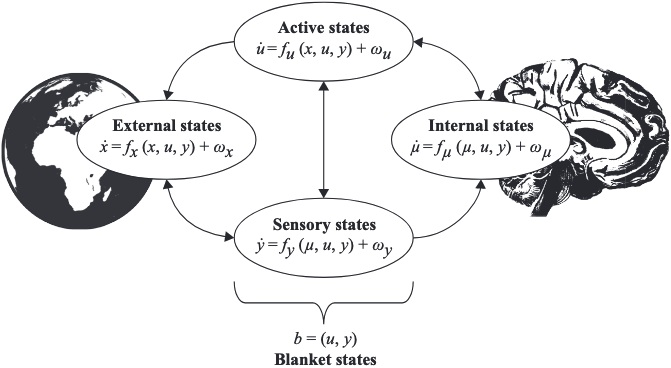
\includegraphics[scale=0.55]{images/markov_blanket.png}
    \caption{Example of a dynamic Markov blanket from \citet{parr2022ActiveInference} which separates an adaptive system, which in this case is a brain, with its environment. The dynamics of each set of states is determined by a deterministic flow specified as a function, $f$. This gives rise to the average rate of change and additional random fluctuations, $\omega$. With arrows indicating the direction of influence between the states.}
    \label{fig:markov_blanket}
\end{figure}

\

The key point is that internal and external states are formally related across the Markov blanket, as both influence and are influenced by the blanket states. Because of this, we can construct conditional probability distributions for the internal and external states, given the blanket states. These distributions are conditioned on the same blanket states, allowing us to associate pairs of expected internal and external states with each other. In other words, on average, internal and external states achieve a form of synchrony. This implies that if we can define independent distributions over external and internal states given their Markov blanket, the two states become informative about each other through the blanket. This synchrony gives internal states the appearance of representing or modelling external states.

\

From a Bayesian perspective, the dynamics of the internal states correspond to a form of approximate Bayesian inference about external states \citep{parr2022ActiveInference}. Since as sensory states change, the associated internal representation is updated through an implicit model of how sensory states are generated. However, the agent’s model cannot simply mimic external dynamics, as this would cause the agent to dissolve into the external environment — similar to why we introduced the concept of a Markov blanket. Instead, the model must encode a preference for certain sensory states. These preferences can be specified in terms of more likely states in the model’s prior distribution. Under this formulation, optimal behaviour — relative to the agent's prior preferences — can be viewed as the maximisation of model evidence through perception and action \citep{parr2022ActiveInference}. This suggests that the system engages in \textit{self-evidencing} \citep{hohwy2016evidencing}, meaning the system acts to acquire sensory states that align with its internal model, thereby maximising model evidence. We will return to the notion of self-evidencing later in this section. 


\subsubsection{Random dynamical system}

While noting that this Markov blanket is indeed necessary for a biological system's persistence over time - the question that we posed initially is what must a system be \textbf{doing} to ensure its persistence over time. Our hypothesis for this was the system was required to keep certain internal parameters within small viable bounds. We can formalise this by describing the system and the sensory states as a random dynamical system. 

\

A random dynamical system consists of two components: a \textit{base flow} and a \textit{dynamical system} on some physical space $X \in \R^d$.

\

The base flow, $\vartheta: \Omega \to \Omega$, is comprises measure-preserving measurable functions: $\vartheta_t: \Omega \to \Omega$ for each time $t \in \R$. These functions form a group of transformation of a probability space $(\Omega, \beta, P)$, such that $(\Omega, \beta, P, \vartheta)$ is a measure preserving dynamical system with $\sigma$-algebra $\beta$ defined on $\Omega$ and $P: \beta \to [0, 1]$ is a probability measure.

\

The dynamical system $(R^d, \varphi)$ comprises of a solution operator: $\varphi: \R \times \Omega \times X \to X$. Which is a measurable function that maps to the metric state space $X \subseteq \mathbb{R}^d$. This function satisfies the \textit{cocycle} property: $\varphi(\tau, \vartheta_t(\omega)) \circ \varphi(t, \omega) = \varphi(t + \tau, \omega)$. This solution operator can be considered as the solution $x(t) = \varphi(t, \omega)(x_0)$ to a stochastic differential equation of the form:

\begin{equation}
	\begin{aligned}
		\dot{x}(t) &= f_X(x) + g_X(x)\omega(t) \\
		x(0) &= x_0
	\end{aligned}
\end{equation}

In all following derivations, we denote random dynamical systems as a tuple: $m = (\R^d, \varphi)$.

\

Crucially, we allow for a partition of the state space $X = R \times S$ , where $R \subset X$ is distinguished by  the existence of a map $\varphi_R : R \times X \to R$ that precludes direct dependency on the base flow. In this  sense, $R$ constitutes an internal state space, while $S \subset X$ constitutes an external state space. Which we allow to give rise to the external mapping: $\varphi_S: \R \times \Omega \times A \times S \to S$. That may only depend on a subset of internal states $A \subset R$. 

\

In this set up, internal states have dynamics that depend on external states and themselves, while external states depend on internal states and themselves but are also subject to fluctuations. See Figure \ref{fig:random_dynamical_system} for a representation of these dynamics.

\begin{figure}[htbp]
    \centering
    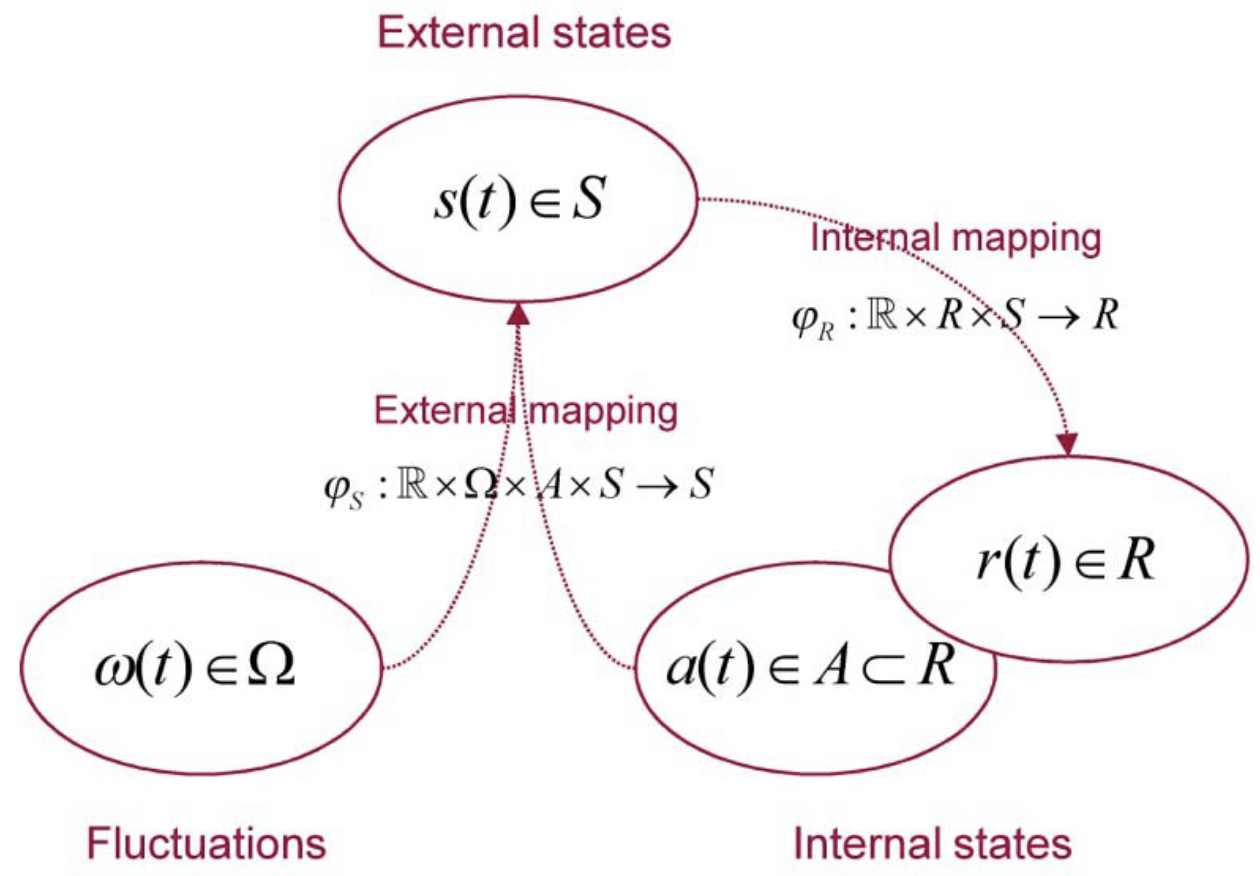
\includegraphics[scale=0.55]{images/random_dynamical_system.png}
    \caption{Image from \citet{friston2012free} depicting the component of described random dynamical system.}
    \label{fig:random_dynamical_system}
\end{figure}

\paragraph{Remark} The use of external states and internal states here is done to be consistent with \citet{friston2012active}. There may be some confusion, as "external states" described in this dynamical system can be more closely associated with "sensory states" in the Markov Blanket (Figure \ref{fig:markov_blanket}).

\

We are interested in biological systems in this discussion thus we can regard the external states $s(t) = \varphi_S(t, \omega)(x_0)$ as the state of the sensory receptors, while the internal states $r(t) = \varphi_R(t)(x_0)$ that include $a(t) \in A \subset R$, respond to sensory perturbation. We will refer to $a(t)$ as active states since they control how environmental fluctuations are sampled by sensory states.

\

We aim to study systems whose physical states, $x(t) = \varphi(t, \omega)(x_0)$, are confined to a bounded subset of states and remain there indefinitely. This is what we have defined as necessary for a system's persistence. Within random dynamical systems, this means the system possesses a random dynamical attractor, which we assume is ergodic. This is a compact set $\mathcal{A}(\omega) \subset X$ which. is invariant under the flow map such that  $\varphi(t, \omega)(\mathcal{A}(\omega)) = \mathcal{A}(\vartheta_t(\omega))$. In terms of ergodic theory, this means there is a unique and stationary ergodic density $p(x | m)$ that is proportional to the amount of time each state is occupied. This density can then be characterised by:

\begin{equation}\label{eq:ergodic_density}
	p(s | m ) = \lim_{T \to \infty} \frac{1}{T} \int^T_0 \delta( x - x(t)) \ dt \ a.s
\end{equation}

The ergodic density $p(x | m)$ is an invariant probability measure that can be regarded as the  probability of finding the system in any state when observed at a random point in time. The existence of the ergodic density and its underlying attractor ensures the system has invariant characteristics that  underwrite its existence over time. 

\subsubsection{Active states and principle of least action}

\begin{definition}[Active System]\label{def:active_system}
	An ergodic dynamical system $m = (\R^d, \varphi)$ is said to be active if it possesses an internal map that satisfies the (locally) extremal condition:
	\begin{equation*}
	\begin{aligned}
		\varphi_R^*= \text{argmin}_{\varphi_R} H(S | m) \\
		H(S | m) = - \int p(s | m)\ln p(s | m)
	\end{aligned}
	\end{equation*}
\end{definition}

In other words, the internal states of an active system minimise the entropy over the external states. Which means that internal states of an active system minimise the dispersion of their external states. Which gives a formal representation of the hypothesis stated at the beginning of this section. The final link that is needed is between surprise and active systems. This link is found in the Principle of Least Action:

\begin{theorem}[Principle of Least Action]\label{theorem:principle_of_least_action}
The internal states of an active system minimise the Lagrangian or surprise, $\mathcal{L}(s(t))$, such that the variation $\delta_t \mathcal{S}$ of action $\mathcal{S}$ with respect to its internal states vanishes $r(t) \in R$ vanishes.
$$
\begin{aligned}
r(t) & =\varphi_R^*(t)\left(x_0\right)=\arg \min _r \mathcal{L}(s(t)) \iff \partial_r \mathcal{L}(s(t))=0 \iff \delta_r \mathcal{S}=0 \\
\mathcal{S} & =\int_0^T \mathcal{L}(s(t)) \ dt
\end{aligned}
$$
\end{theorem}

\begin{proof}
	We can relate the entropy of the ergodic density $P(s(t) | m)$ in an active system using the ergodic theorem:
	
	$$
	H(S | m) = - \int p(s | m)\ln p(s | m) = - \lim_{T \to \infty} \frac{1}{T} \int_0^T dt \ln p(s(t) | m) = \lim_{T \to \infty} \frac{1}{T} \int_0^T \mathcal{L}(s(t)) \ dt
	$$
	
	This means that for large enough $T$, we can specify:
	
	$$
	T \mathcal{H}(S | m) = \int_0^T \mathcal{L}(s(t)) \ dt = \mathcal{S}
	$$
	
	This equivalence means that $\delta_r\mathcal{S} = 0 \iff \delta_r\mathcal{H}(S | m) = 0 \iff \text{argmin}_{\varphi_R} H(S | m)$. Moreover, $\partial_r \mathcal{L}(s(t)) = 0 \iff \delta_r \mathcal{S} = 0$ by the  fundamental Lemma of variational calculus.
\end{proof}

Since we have assumed that active states, $a(t)$, are a subset of the internal states of the biological system. The Principle of Least Action can be summarised as saying that a biological system minimises the surprise of sensory states by adjusting its internal states, including active states. Which means that an active biological system is performing active inference. 

\subsubsection{Remark on the relation to Free Energy Principle}

The previous derivations are based on \citet{friston2012active}. Active inference is defined differently in this thesis. It is derived as a Corollary to the \textit{Free Energy Principle}. The derivation of active inference in this regard bears a close relation to (approximate) Bayesian inference and variational free energy derivation of active inference that will be done along the ``low road''. Although, we have completed our goal to show that a persistent biological system must be conducting active inference - we will finish this section true to \citet{friston2012free} and that definition of active inference.

\subsubsection{Free Energy Principle and Active Inference}

The fundamental issue with our current formulation is how internal states can minimise surprise given that they do not know the effect they will have on external states. We have answered \textbf{why} this is required, but we have not discussed \textbf{how} it can be done.

\

Intuitively, the solution regards the system as optimising a probabilistic model of the external dynamics, which is used to minimise surprise. This solution was mentioned in the previous section on Markov blanket when it was remarked that internal states create some implicit model of the external states through the conditioning on the blanket. z

\begin{definition}[Generative Model]\label{def:generative_model}
Let $p(s(t)|m)$ be defined as in Definition \ref{def:active_system}, be expressed in terms of some arbitrary parameters $\psi(t) \in \Psi$ that are themselves random variables. We define the generative model as:

\begin{equation*}
	\begin{aligned}
		p(s(t), \psi(t)) &= p(s(t)|\psi(t))p(\psi(t)) \\
		p(s(t)) &= \int_\Psi p(s(t), \psi(t)) d\psi
	\end{aligned}
\end{equation*}
\end{definition}

Where $p(s(t))$ is called the marginal likelihood. 

\

Further, we define the proposal distribution, $q$, which plays the role of an arbitrary probability density over the parameters of the generative model. The probability density is parameterised by some subset of the internal states of the system, $\mu(t)$. Crucially, this proposal density is over the variables that parameterise the marginal likelihood of the external states. This allows us to define free energy for a biological system:

\begin{definition}[Proposal Distribution]\label{def:proposal_distribution}
Let $q(\psi(t) | \mu(t))$ denote a mapping $q: R \times \Psi \times R \to R$. This serves as an arbitrary probability density defined over the parameters of the generative model called the proposal density. Further let this density be parameterised by $\mu(t) \in R$ with $\mu(t) \subset r(t)$. 
\end{definition}

A point to note is that $\psi \in \Psi$ are not observable quantities. They are induced with a proposal density and only exist to parameters the marginal likelihood of external states. This quantities are often referred to as \textit{hidden states}.

\begin{definition}[Free Energy]\label{eq:free_energy}
Free energy is now defined in terms of the proposal and generative  densities as the following expectation:
$$
F(x(t)) = \int_\Psi q(\psi(t) | \mu(t))\ \ln\frac{q(\psi(t) | \mu(t))}{p(s(t), \psi(t))} d\psi
$$
\end{definition}

Equipped with these components we now define the Free Energy Principle as: 

\begin{theorem}[Free Energy Principle]\label{theorem:free_energy_principle}
Let $ m = (\R^d, \varphi)$ be an ergodic random dynamical system with state space $X = R \times S \in \R^d$. If the internal states $r(t) \in R$ minimise free energy then the system conforms to the principle of least action and is an active system. By the principle of least action \refp{theorem:principle_of_least_action}:

$$
r(t) = \varphi_R^*(t)(x_0) = \text{argmin}_{r} \mathcal{F}(x(t)) \Rightarrow \delta_r \mathcal{S} = 0 \\
$$
\end{theorem}

\begin{proof}
	We can express Free Energy as:
	\begin{equation}\label{eq:free_energy_decomposition}
	\begin{aligned}
		F(x(t)) &= \int_\Psi q(\psi(t) | \mu(t))\ \ln\frac{q(\psi(t) | \mu(t))}{p(s(t), \psi(t))} d\psi \\
		&= \int_\Psi q(\psi(t) | \mu(t))\ \ln\frac{q(\psi(t) | \mu(t))}{p(\psi(t) | s(t), m)} d\psi - \ln p(s(t) | m) \\
		&= \mathcal{L}(s(t)) + D_{KL}\left[ \psi(t) | \mu(t) \| p(\psi(t) | s(t), m) \right]
	\end{aligned}
	\end{equation}
	By Gibbs' inequality, $D_{KL} \geq 0$, therefore free energy is minimised with respect to $\mu(t) \in R$ when the KL-Divergence is 0 (If such a solution exists). This means that $\mathcal{F}(x(t) = \mathcal{L}(s(t))$ and its variation with respect to $a(t) \in R$ vanishes:
	
	$$
	a(t) = \text{argmin}_a\mathcal{F}(x(t)) \Rightarrow \partial_a \mathcal{F}(x(t)) = 0 \Rightarrow \partial_a \mathcal{L}(s(t)) = 0 \Leftrightarrow \delta_a \mathcal{S} = 0
	$$
	
	From \refp{theorem:principle_of_least_action} we see that surprise does not depend on $\mu(t)$, which means $\partial_\mu \mathcal{L}(t) = 0 \Leftrightarrow \delta_\mu \mathcal{S} = 0$ and therefore $\delta_r \mathcal{S} = 0$.
	

\end{proof}

\paragraph{Remark} In this proof, we have claimed that when minimised the KL-Divergence between the conditional distribution and proposal density is zero. This rests on the assumption that the proposal density can have the same form as the conditional density. This corresponds to \textit{exact} Bayesian inference. When this assumption is relaxed - free energy becomes an upper bound on surprise and the inference is \textbf{approximately} Bayesian. 

\begin{corollary}[Bayesian inference]\label{cor:bayesian_inference}
	Systems that conform to the free energy principle represent the causes of their sensory states in a Bayesian sense: This follows from \refp{eq:free_energy_decomposition}, where minimising free energy with respect to the internal states minimises the divergence between the proposal density and the posterior density over the parameters of the likelihood function:
	
	\begin{align*}
		\mu(t) & =\arg \min _\mu \mathcal{F}(x(t)) \\
		& =\arg \min _\mu D_{K L}(q(\psi(t) \mid \mu(t)) \| p(\psi(t) \mid s(t), m))
	\end{align*}
\end{corollary}

In other words, the optimal proposal density $q(\psi(t) \mid \mu(t))$ - parameterised by internal states becomes the posterior $p(\psi(t) \mid s(t), m)$, under the model entailed by the system.

\begin{corollary}[Active Inference]
	Systems that conform to the free energy principle will selectively sample what they 'expect to see'. This follows from a final rearrangement of free energy in terms of complexity and accuracy or the log likelihood of sensory states under the proposal density:
	
	\begin{align*}
	\mathcal{F}(x(t)) & =\int_{\Psi} q(\psi(t) \mid \mu(t)) \mathcal{L}(s(t)) d \psi+\int_{\Psi} q(\psi(t) \mid \mu(t)) \ln \frac{q(\psi(t) \mid \mu(t))}{p(\psi(t) \mid s(t), m)} d \psi \\
		& =\int_{\Psi} q(\psi(t) \mid \mu(t)) \ln \frac{q(\psi(t) \mid \mu(t))}{p(\psi(t) \mid s(t), m) p(s(t) \mid m)} d \psi \\
		& =D_{K L}(q(\psi(t) \mid \mu(t)) \| p(\psi(t) \mid m))-\int_{\Psi} q(\psi(t) \mid \mu(t)) \ln p(s(t) \mid \psi(t), m) d \psi \\
		a(t) & =\arg \min _a \mathcal{F}(x(t)) \\
		& =\arg \max _a \int_{\Psi} q(\psi(t) \mid \mu(t)) \ln p(s(t) \mid \psi(t), m) d \psi
\end{align*}

\end{corollary}


This is called active inference and manifests as a selective sampling of (typical) sensory states that are most likely under the system's posterior beliefs, by Corollary \refp{cor:bayesian_inference}.

\subsection{Low Road to Active Inference}

Humans and other animals live in a world of sensory uncertainty. Through, introspection may tell us that perception is deterministic, many factors contribute to limiting the reliability of sensory information about the world. For example the mapping of 3D objects into a 2D image, neural noise introduced in early stages of sensory coding, and structural constraints on neural representations and computations \citep{knill2004bayesian}. Our brains must effectively deal with the resulting uncertainty to generate perceptual representations of the world and to guide our actions.

% This naturally to the idea that perception is a process of unconscious, probabilistic inference \citep{helmholtz1867concerning}. 

\

With aid from advances in artificial intelligent - researchers have begun to rigorously apply concepts of probability theory into perception. \citep{knill2004bayesian} One striking observation from this work is the ways in which human observers behave as Bayesian optimal observers. A correspondence which has fundamental implications for neuroscience, particularly for neural representations of cortical functions like perception and learning. \citep{trommershauser2003statisticalb, trommershauser2003statisticala}

\subsubsection{Hallucinations in perception}

One of the earliest and perhaps most well-known investigations into hallucinations in perception was conducted by Wilder Penfield. \citep{penfield1961activation} Penfield suggested that the cortex is capable of producing percepts based on past experiences, even in the absence of current sensory input. He referred to the temporal lobes as the ``interpretive cortex,'' believing that this region was responsible for interpreting the world through past experiences, based on his observations of the temporary hallucinations induced by electrical stimulation. These hallucinations often included familiar voices, musical tunes, or the sight of objects, which seemed to the patients like flashbacks from their past. The subjects' feedback led Penfield to believe that these memories were experienced within a brief episodic context, placed either in the present or the past. Hence, he coined the term interpretive cortex. \citep{knill2004bayesian}

\

Penfield was reluctant to definitively state whether the memories themselves or merely their interpretations were elicited by the electrical stimulation of the temporal cortex. However, the most parsimonious interpretation suggests that memories of sounds, objects, or people are distributed across the cerebral cortex rather than being stored in a specific region. The medial temporal lobes, including the hippocampus, play a key role in organising these distributed memories. \citep{aggelopoulos2015perceptual} Moreover, under certain conditions, such as electrical stimulation, these memories can be as vivid as actual sensory input. When the hallucinated object and context conflicted with available sensory input, a distorted percept was reported, indicating that a process of evaluation, as proposed by Helmholtz, was at play.

\

Helmholtz’s theory of unconscious inference posits that perception is not a mere reflection of sensory input but involves experiential data that may not be represented in the immediate stimulus. \citep{helmholtz1867concerning} Elements not represented in the current stimulus are inferred from past experiences, leading to perception as a constructed interpretation of the world. This explains how false percepts, such as hallucinations, can occur when the brain uses past experiences to interpret incomplete or ambiguous sensory data.


\subsubsection{Perceptual Inference}

The link between past experiences and sensory stimuli is also evident in neural activity. \citet{ishai2000distributed} presented fMRI evidence suggesting that mental imagery of familiar memories activates subsets of the regions involved in object perception. Notably, in this and other fMRI studies involving objects, faces, and other complex, ecologically meaningful stimuli, the activation of striate and peristriate cortical areas was not significantly higher than that elicited by scrambled visual stimuli. This suggests that coherent stimuli engage higher-order processing beyond early visual areas.

\

Additionally, another fMRI study on adult humans indicated that visual memories may be stored in areas like the temporal and fusiform gyri, which are closely linked to the perception of these stimuli \citep{sterpenich2007sleep}. This evidence supports the hypothesis that the perception of ecologically meaningful stimuli relies on cortical regions that are also activated during the imagery of memories, particularly in the temporal lobes. Thus, declarative visual memories formed through experience may be stored in the same neurons or networks responsible for perceiving object features. Without these memories, relevant features or objects might not be perceptible. In other words, perception is not just a passive process but one that draws on stored memories to interpret incoming stimuli.

\paragraph{Forward Models}

A key concept in active inference is that systems actively engage with their environment, and the sensorimotor system plays an important role in this process. \citet{miall1996forward} proposed a forward model to explain how the brain integrates sensory and motor information. This model predicts the next state of the motor system based on current sensory input and motor commands.

\

Other studies suggest that the cerebellum, traditionally associated with motor control, is also involved in cognitive processes such as conditional learning, reward processing, and the sense of agency. \citep{welniarz2021forward} This cognitive function allows us to recognise actions as our own, further reinforcing the cerebellum’s role as a bridge between sensorimotor function and cognition. Anatomically, the cerebellum is well positioned to integrate sensory and motor information through its connections with cerebral, striatal, and spinal systems. This makes it an essential part of the brain’s forward modelling system, allowing it to predict and compare outcomes, thereby supporting both motor control and higher cognitive processes.

\subsubsection{Bayesian Brain}

So far, we have discussed perception as a process of inference, extending this idea to the sensorimotor system through the concept of a forward model. We can now deepen this discussion by examining forward models from a Bayesian perspective. In the context of active inference, the forward model is referred to as the \textit{generative model}. This generative model represents a probability distribution over the environment's \textit{hidden states}, $x$, and observations, $y$, denoted as $p(x, y)$. It plays a central role in the brain’s inferential processes, allowing the system to predict and update its beliefs about hidden states based on incoming sensory data.

\

The generative model represents how sensory data, $y$, could be generated from hidden states, $x$. This is conceptually similar to the \textit{generative process} (see Figure \ref{fig:generative_process}). However, the generative process refers to the true causal structure by which sensory data is actually generated. In this process, the hidden states, $x^*$, generate observations, $y$, which are then used to infer the hidden states, $x$, within the model. These two hidden states - $x^*$ and $x$ - are distinct. The generative model involves a set of hypothesised hidden states that may not include the actual values of the hidden states in the real world. In other words, the brain’s models of the environment may infer hidden states that do not exist outside the mind, and vice versa \citep{parr2022ActiveInference}.

\begin{figure}[htbp]
    \centering
    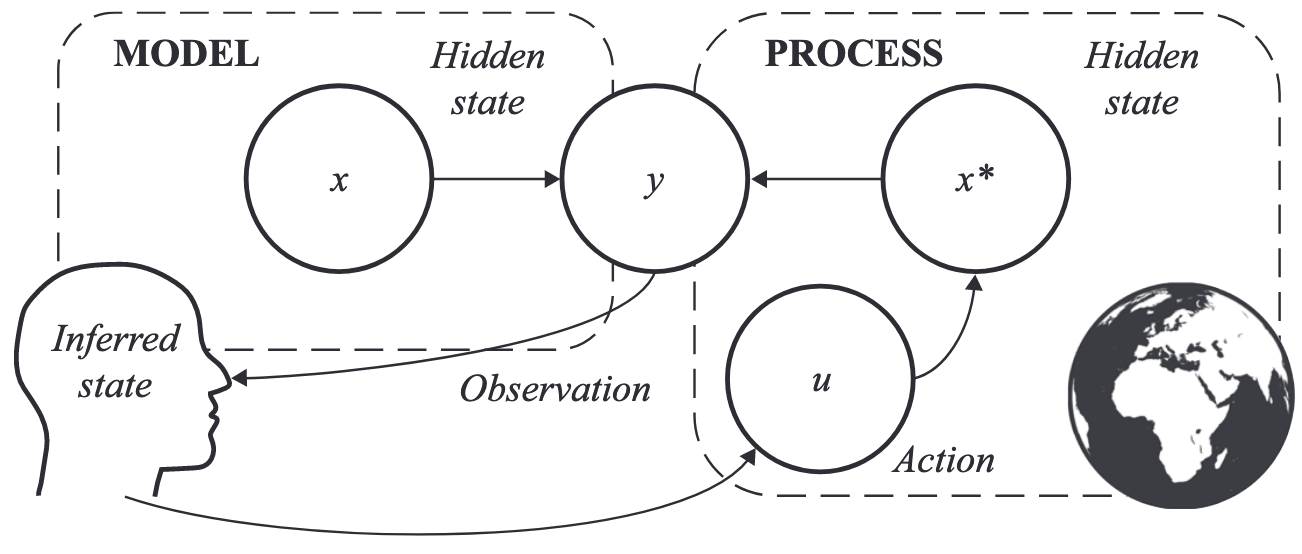
\includegraphics[scale=0.6]{images/generative_process.png}
    \caption{Image from \citet{parr2022ActiveInference} depicting the generative model and process. This depictions shows there are some internal (hidden) parameters of our mode, $x$. Which are inferred by the observations generated by the environment $y$. The central distinction to note is that in theory, there exists some true state of the environment, $x^*$. This is the true causal foundation for observations in the environment. This true state may or may not be with the distribution of states specified by the prior component in the generative model - $P(x)$.}
    \label{fig:generative_process} 
\end{figure}

\subsubsection{Inference and Bayesian Optimality}

The key task in inference is determining the new hidden states of our model given new observations. This is achieved through Bayes' rule:

\begin{align}
	\underbrace{P(x | y )}_{\text{Posterior Distribution}} &= \frac{P(y | x)P(x)}{P(y)} \label{eq:posterior} \\
	\underbrace{P(x, y)}_{\text{Generative Model}} &= \underbrace{P(y | x)}_{\text{Likelihood}}\underbrace{P(x)}_{\text{Prior}} \label{eq:decomposed_generative}
\end{align}

\refp{eq:posterior} shows how Bayes' rule updates our beliefs about the hidden states, $x$, given observations, $y$. \refp{eq:decomposed_generative} decomposes the generative model into the likelihood and prior distributions. Bayesian inference thus centers on obtaining the posterior distribution. The term $P(y)$, known as the model evidence or marginal likelihood, acts as a normalizing constant to ensure the posterior is a valid probability distribution. We will explore its significance and computational challenges in the next section.

\

A few key points in Bayesian inference are worth noting. First, it combines top-down dynamics (via likelihood) and bottom-up priors to update beliefs about hidden states. This can perhaps be seen more clearly in $P(x | y) \propto P(y | x)P(x)$. These dynamics directly linking our earlier discussion on perception.

\

Second, Bayesian inference is considered optimal. In the context of our discussion on combining both bottom-up and top-down dynamics in the brain, the quantity with respect to which Bayesian inference is optimal should reflect these dynamics. And indeed, optimality is achieved with respect to \textit{variational free energy} (VFE), a concept originating from statistical physics \citep{friston2006free}. Which we will see in the next section does indeed fulfil our description. By evaluating the full distribution over hidden states, Bayesian inference effectively handles uncertainty, mitigating the shortcomings of approaches that only rely on single point estimates.

\

It is important to emphasise that this optimality is inherently \textit{subjective} - it depends on the generative model being used. The generative model may or may not include the actual hidden state of the environment, $x^*$, assuming such a true state exists. In other words, the brain's model of the world is limited by its capacity to represent the true causal dynamics of the environment. Therefore, the brain’s performance in managing the integration between the top-down and bottom-up dynamics is constrained by the choice of its generative model. If the model fails to capture important features of the environment, its predictions will be less accurate, but Bayesian inference will be optimal within the bounds of the chosen model.

\subsubsection{Minimising Variational Free Energy}

%TODO: Define the surprise 

The two points of discussion that were postponed in the previous section were the marginal likelihood in Bayes' rule and variational free energy. And indeed, this two items are closely related.

\

The fundamental issue with Bayesian inference is the computation of the marginal likelihood or model evidence in the expression of the posterior distribution \refp{eq:posterior}. Computing the marginal likelihood requires us to marginalise, or integrate, our the hidden state in the generative model:

\begin{equation}
	P(y) = \int P(x, y) \ dx
\end{equation}

Firstly, This computation may require the integration of \textit{analytically} intractable integrals. Secondly, for anything by trivial state spaces, the integral over the entire space will be \textit{computationally} intractable. To resolve this issue, we refer to a scheme of approximate Bayesian inference - \textit{variational inference}. Variational inference casts the inference problem as an optimisation problem, but doing we are able to find a tractable approximate Bayesian posterior, called the \textit{variational posterior distribution}. The optimisation is done with respect to the variational free energy.

\begin{figure}[htbp]
    \centering
    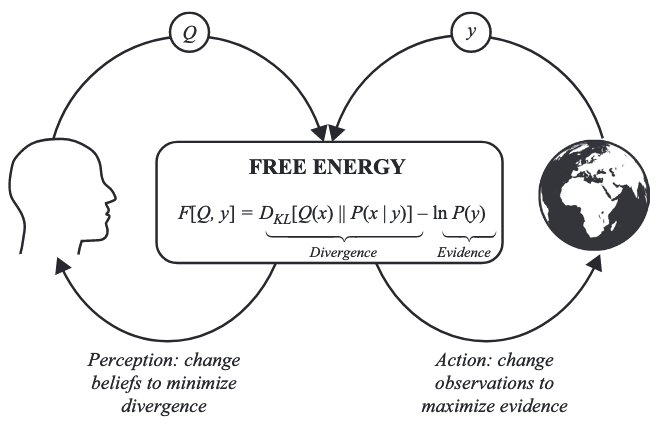
\includegraphics[scale=0.55]{images/vfe_minimisation.png}
    \caption{\citet{parr2022ActiveInference}}
    \label{fig:vfe_minimisation}
\end{figure}


\begin{definition}[Variational Free Energy]\label{def:variational_free_energy}
Let the generative model, $p$, and variational distribution, $q$, be parameterised by $\theta$ and $\phi$ respectively. Then we define variational free energy (VFE) as:
	$$
	\mathcal{F}(q, y) =  \int q(x; \phi) \ln \frac{q(x; \phi)}{p(x, y; \theta)}
	$$
\end{definition}

The variational inference scheme initialises the variational distribution as some distribution over the hidden states. The choice of the form of this posterior is again subjective and will change the inference dynamics. We will then adjust the parameters of the variational distribution so as to minimise variational free energy.

\

We can demonstrate the optimality claim of Bayesian inference by decomposing VFE as: 

\begin{equation}\label{eq:vfe_low_road}
	\begin{aligned}
		\mathcal{F}(Q, y) &=  \int Q(x; \phi) \ln \frac{Q(x; \phi)}{P(x, y; \theta)} \\
		&= - \ln P(y; \theta) + \int Q(x; \phi) \ln \frac{Q(x; \phi)}{P(x | y; \theta)} \\ 
		&= - \underbrace{\ln P(y; \theta)}_{\text{Evidence}} + \underbrace{D_{KL}\left[ Q(x; \phi) \,\|\, P(x | y; \theta) \right]}_{\text{Divergence}}
	\end{aligned}
\end{equation}

By Gibbs' inequality, $D_{KL} \geq 0 $, further we can note that if $Q(x; \phi) = P(x | y; \theta)$ then $D_{KL} = 0$. Therefore, we can see that the true Bayesian posterior is indeed optimal with respect to VFE. Moreover, we see that VFE is a function of both the variational distribution and of the data. This demonstrates a fundamental tenet of active inference that we can both change our beliefs of the environment to minimise surprise, as well as take action on the environment to minimise surprise of the observations. We have not linked VFE to surprise, which we will do in the next section. See Figure \ref{fig:vfe_minimisation} for a representation of this. 

\

Further, our intuition for the quantity that is optimal under Bayesian inference is there should be the presence of top-down and bottom-up dynamics. Indeed, we can see these dynamics reflected in an alternative decomposition of VFE:

\begin{equation}
\begin{aligned}
	\mathcal{F}(Q, y) &=  \int Q(x; \phi) \ln \frac{Q(x; \phi)}{P(x, y; \theta)} \\ 
	&= \underbrace{D_{kl}\left[ Q(x; \phi) \| P(x; \theta)  \right]}_{\text{Complexity}} - \underbrace{\mathbb{E}_{Q(x)}\left[ \ln P(y | x; \theta) \right]}_{\text{Accuracy}}
\end{aligned}
\end{equation}

We can notice smaller the change to the prior beliefs of the hidden states gets rewarded under the objective of VFE minimisation. While, the accuracy term rewards change to the internal states that better reflect the sensory data. This highlights the tradeoff between prior experience and new sensory stimuli that we outlined during this section.

\subsubsection{Minimising Surprise}

We aim to show that the brain, under the hypotheses of perception as inference, is performing active inference. By our definition, this requires us to show that the brain is actively perceiving and acting to as to minimise the surprise of observations generated from the environment. Surprise (also called surprisal) in the context of probability and information theory has formal definition:

\begin{definition}[Surprisal]\label{eq:surprisal}
	$$\mathcal{I}(y) = - \ln P(y)$$
\end{definition}

This definition makes sense with our own notion or surprise. If we believe an observation to be `unlikely', let us say that under our generative model $P(y_1) = 0.1$, then the surprise of the observation is $ \mathcal{I}(y) \approx 2.3$ nats. \footnote{Like bits, nats are units of information. The choice of unit depends on whether we use a logarithm to the base 2 (bits) or a natural logarithm (nats).} While, say $P(y) = 0.8$ then $\mathcal{I}(y) \approx 0.1$ nats. 

\

Thus, we aim to show that through both perception and action the brain (under the assumptions made in this chapter) is performing active inference, that is, that the brain is minimising the surprisal of the sensory observations of the environment. In fact, we have already shown this. Consider the final line in \refp{eq:vfe_low_road}. 

\begin{equation}
	\begin{aligned}
		\mathcal{F}(Q, y) &= - \ln P(y; \theta) + D_{KL}\left[ Q(x; \phi) \| P(x | y; \theta) \right] \\
		&\geq - \ln P(y; \theta) \\
		&= \mathcal{I}(y)
	\end{aligned}
\end{equation}

This demonstrates is that VFE is an upper bound on surprise. Therefore, the minimisation of VFE will result in the minimisation of surprise. Further, as we argued in the previous section, minimising VFE can be done by changing our beliefs to better reflect the environment, as well as changing the environment to reflect our beliefs. These are the conditions that we required to justify the brain performing active inference. 

\subsubsection{Expected Free Energy}

While we have justified the brain's engagement in active inference, we must also recognize a fundamental \textit{prospective} aspect of cognition: \textit{planning}.

\

In active inference, a sequence of actions is referred to as a \textit{policy}. It is important to distinguish between actions, which directly influence the external world, and policies, which represent behavior patterns. Planning is thus treated as an inference problem, aligning with the Bayesian approach we have followed. To do so, we must define priors and likelihoods.

\

Future observations resulting from a particular policy are unknown, as they have not yet occurred, and must be predicted by the generative model. This prediction relies on two components: first, our belief about how hidden states evolve under a policy, denoted by $P(\tilde{x} | \pi)$, where $\tilde{x}$ represents a trajectory of hidden states. Second, the likelihood distribution, $P(y | x)$, describes the expected observations given hidden states. These two components enable the brain to simulate the counterfactual consequences of its actions, akin to asking: “What happens if I do this?” By marginalizing over hidden states, we obtain the marginal likelihood (or its free energy approximation), $P(\tilde{y} | \pi)$, which reflects the evidence for a policy.

\

Active inference breaks planning into two steps: first, assigning a score to each policy, and second, forming posterior beliefs about which policy to pursue. The prior belief about which policy to follow depends on its score, where better policies are assigned higher probabilities. In active inference, the score of a policy is the negative expected free energy, $\mathcal{G}$, which differs from the variational free energy $\mathcal{F}$. While $\mathcal{F}$ is based on present and past observations, $\mathcal{G}$ considers future observations that depend on the policy.

\

Expected free energy evaluates the generative model’s prediction of future outcomes under a given policy, extending to a planning horizon. Since policies unfold over multiple time steps, the final measure of expected free energy integrates over future steps. The negative expected free energy can then be converted into a policy score, with policies minimising expected free energy assigned higher probability. This reflects a prior belief about which policy the agent is likely to pursue. Ultimately, inferring a particular policy affects the predictions of future sensory data.

\subsubsection{Computing EFE}

We have assumed that during planning, the organism scores its policies according to their expected free energy. However, we have not yet defined what expected free energy is:

\begin{equation}\label{eq:efe}
	\begin{aligned}
		\mathcal{G}_\pi &= \int Q(\tilde{x}, \tilde{y} | \pi) \ln \frac{Q(\tilde{x} | \pi)}{P(\tilde{x}, \tilde{y} | \pi)} & \text{(L1)}\\ 
		&= \mathbb{E}_{Q(\tilde{x}, \tilde{y} | \pi)} \left[ \ln \frac{Q(\tilde{x} | \pi)}{P(\tilde{x}, \tilde{y} | \pi)} \right] & \text{(L2)} \\
		&\approx \mathbb{E}_{Q(\tilde{x}, \tilde{y} | \pi)} \left[ \ln Q(\tilde{x} | \pi) - \ln Q(\tilde{x} | \tilde{y}, \pi) \right] - \mathbb{E}_{Q(\tilde{y} | \pi)}\left[ \ln P(\tilde{y} | C) \right] & \text{(L3)}\\
		&= - \underbrace{\mathbb{E}_{Q(\tilde{x}, \tilde{y} | \pi)} \left[ \ln Q(\tilde{x} | \tilde{y}, \pi) - \ln Q(\tilde{x} | \pi) \right]}_{\text{Epistemic}} - \underbrace{\mathbb{E}_{Q(\tilde{y} | \pi)}\left[ \ln Q(\tilde{y} | C) \right]}_{\text{Pragmatic}} & \text{(L4)}\\ 
	\end{aligned}
\end{equation}


The definition of EFE in (L1) is identical to the definition of VFE in \refp{eq:vfe_low_road}, except for the first variational posterior distribution term including the observations as well as $\tilde{x}, \tilde{y}$ representing a trajectory. The observations can then enter the expectation in (L2). This makes sense since we are considering observations that have not occurred yet. (L3) is a fundamental step in active inference, first we replace the true posterior with our variational posterior ($P(\tilde{x} | \tilde{y}, \pi) \to Q(\tilde{x} | \tilde{y}, \pi)$). Second, we drop the condition on $\pi$ in the second term, instead we condition on some distribution that is used to encode the preferences of the system, $C$. This means the system seeks to find policies expected to produce those observations. The agent’s preferences can be independent of the policy being followed, which allows us to drop the condition on $\pi$. 

\

(L4) labels two terms that underscore active inference's appeal in planning. The first term is the epistemic term, notice that this term is negated, thus to minimise EFE, we need to maximise this epistemic term. What this term is representing is the difference between the variational distribution prior and conditional on an observation. That is - the agent is driven to seek out observations that reduce uncertainty about hidden states \citep{smith2022} The second term is the pragmatic term which as mentioned allows us to score the observations with respect to the agent's preferences. 

\section{Applications}

%TODO: I need to draw a line here between the hypothesis and falsifiability of the coming descriptions. 

In this section, we aim to complement the preceding section's conceptual treatment of active inference we use the theory we have put in place in the first section into practice. We aim to demonstrate how active inference and other computation neural models are to be build to solve planning and control problems. 


In each of the subsequence subsections we will be presenting a model, discussing its biological plausibility and testing that model in an environment. Each model will be tested in a Markov Decision Process (MDP), specifically these it will be a partially observable MDP (POMDP). 


%TODO: Still need to get far more precise with this section - not urgent but needed

\subsection{Markov Decision Processes}

Markov decision processes are sequential models for decision making when the outcome of those decision is not certain. The MDP framework has been used in a variety of fields, such as ecology, economics and reinforcement learning.

\begin{definition}
	A Markov Decision Process is defined as a 4-tuple: $(S, A, P_a, R_a)$
	\
	\begin{itemize}
		\item S - is the state space
		\item A - The space of action that the agent can take
		\item $P_a$ - This can be understood as the state transition from time $t$ to $t+1$ by taking action $a_t$ in state $s_t$: $P(s_{t+1} | s_t, a_{t})$
		\item $R_a$ is the immediate reward that is observed after transitioning from states $s_t$ to $s_{t+1}$ 
	\end{itemize}
\end{definition}


MDP refers to the underlying structure of state transitions that still follow the Markov property. The process is called a "decision process" because it involves making decisions that influence these state transitions, extending the concept of a Markov chain into the realm of decision-making under uncertainty.

\

In the context of our generative model, this allows us to factorise the model for more efficient probabilistic inference. We assume that the generative model is the joint distribution over all observations, states and actions up until sometime horizon $T$:

\subsection{Predictive Coding}\label{section:predictive_coding}

We will now move our implementation of active inference into continuous state spaces. We present an active inference agent with a \textit{predictive coding} inspired generative model. This implementation will take a somewhat different approach to the others. It will take the form of a tutorial on the predictive coding model similar to what is done in \citet{bogacz2017tutorial}.

\

Predictive coding presents a theory of cortical function - namely, that the core function of the brain is to minimise prediction error. The intuition behind this is that the brain is comprised of a hierarchy of neurons making predictions about the activity of the neurons in the level below them. \citep{friston2008hierarchical} The prediction error in this case is the difference between the neural activity predicted by the higher level compared to the actual neural activity. Over time, the hierarchy of layers encodes a range of predictions at difference scales, with fine details in local sensory data represented at the lower levels and global invariant properties of the causes of sensory data encoded at higher levels \citep{millidge2021applications}. 

\

These preiction errors are thought to then be propagated up the neural hierarchy and used to make better predictions. In the case of predictive coding - reducing these errors can be done in two main ways. Firstly, through immediate inference about the hidden states of the world, which can be through of as perception. This inference is done in a Bayesian fashion where the prior neural activity of the layer is combined with the residual error of the prediction in order to compute the posterior neural activity. This is done using the processes of variational inference and will be explained fully later in this section.


Secondly, though updating of a model of the world to better explain the observations, which can be understood as learning. A neuron is connected to a neighbouring neuron via something called a synaptic connection. Associated with these are synaptic weights - these weights can be adjusted to strengthen or weaken the connection between two neurons. Thus by adjusting this, we are able to adjust the prediction made about activity in the layer below.

\

Finally, as we have discussed previously, another way to reduce the prediction error is to change the sensory observations to better match the beliefs of the model. This process is not described within the predictive coding framework. Nevertheless, the generative components that are needed for this process are. We will be extending the predictive coding model to include planning by using expected free energy. 

\subsubsection{Origins}

Predictive coding as a neuroscientific theory originated in the 1980s and 1990s, perhaps the most famous paper first describing its use as a model for neural processing was done by \citet{rao1999predictive}. In this, predictive coding was used as a model for visual processing. The model was exposed to natural images, a hierarchical network of model neurons implementing such a model developed simple-cell-like receptive fields. While the neurons encoding the errors\footnote{This model is called "predictive coding" because some of the nodes in the model encode these prediction errors} showed endstopping and other extra-classical receptive-field effects. \citep{rao1999predictive}.

\

Predictive coding in its mathematical form as a comprehensive theory of cortical function was done by \citet{friston2003learning, friston2005theory}. This placed predictive coding and the minimisation of prediction errors as equivalent to minimising free energy under the expectation maximisation scheme. \citep{dempster1977maximum} This will be discussed further in a later section.

\subsubsection{Predictive Coding as Variational Inference}

The modern implementation of prediction coding can be best understood as a variational inference algorithm \citep{millidge2021applications}. What this means is that the predictive coding algorithm defines a generative model. This comprises of a prior and a likelihood distribution which in the case of predictive coding are Gaussian distributions. Further, variational inference requires a variational posterior distribution that is used as the tractable alternative to the Bayesian posterior. Thus, let us define these components for our model.\footnote{We are assuming a single hidden state and a single observation dimension for this section. Hence we define the variance as a scalar value - $\sigma^2$ - , rather than as a matrix - $\Sigma$ - which will be done. Similarly, $x$, $y$ represent scalar values and not vectors. }

\begin{equation}\label{eq:pc_single_model}
    \begin{aligned}
        & q(x ; \phi) = \delta( x - \phi ) &(A) \\
        & y | x \sim N(f(x	; \theta), \sigma^2_y) &(B) \\
        & x \sim N(\bar{\mu}, \sigma^2_x) &(C) \\ 
    \end{aligned}
\end{equation}

(A) - This is our variational posterior distribution. $\delta$ denotes the Dirac-delta distribution which is a point mass probability distribution. The alternative form of the variational posterior is a Gaussian under the Laplace approximation. \cite{friston2003learning} This approximation defines the variance of a Gaussian distribution as a function of its mean. Essentially, allowing us to focus solely on estimating the first moment of the distribution. Both of these forms results in the same variational inference update equations and thus we have chosen the Dirac-delta for simplicity. Predictive coding under the Laplace approximation will be derived in Appendix \ref{appendix:laplace_approx}. 

\

(B) - This is the form of our likelihood distribution. This component represents the beliefs the model has about how sensory observations, $y$, are generated from the hidden state of the model $x$. We are assuming the relation is some function $f$ of the hidden states parameterised by $\theta$. With variance $\sigma_y^2$

\

(C) - This defines the form of our prior beliefs about the hidden variable of our model, $x$. In this case, it is defined as a Gaussian with a mean of $\bar{\mu}$. We will be assuming a value of this when we operationalise this model.

\

We are not able to express the variational free energy that the variational inference aims to minimise using the generative and variational components we have defined. Before doing so, we express the variational free energy as see in 


Having defined each generative component of our model as well as the form of the variational posterior 

Given our definitions of the variational posterior and the generative model, we can concretely write down the form of the variational free energy that will be optimised during inference. First we will define a more convinient form of the VFE in \refp{eq:vfe_low_road}:

\begin{equation}\label{eq:vfe_entropy_energy}
	\mathcal{F} = \underbrace{\mathbb{E}_{q(x ; \phi)} \left[ 	\ln q(x ; \phi) \right]}_{\text{Entropy}} - \underbrace{\mathbb{E}_{q(x ; \phi)} \left[ 	\ln p(y | x ; \theta) p(x) \right]}_{\text{Energy}} \\
\end{equation}

This is a useful form since we need only consider the energy term since the entropy of a Dirac-delta distribution is 0.

\begin{equation}\label{eq:pc_vfe}
	\begin{aligned}
	& \mathbb{E}_{q(x ; \phi)} \left[ 	\ln p(y | x ; \theta) p(x) \right] \\
	&= \int \delta(x - \phi) \ln \left( \mathcal{N}(y ; f(x; \theta), \sigma^2_y) \ \mathcal{N}(x; \bar{\mu};, \sigma^2_x) \right) dx \\
		&= \ln \mathcal{N}(y; f(\phi; \theta), \sigma^2_y) + \ln \mathcal{N}(\phi; \bar{\mu}, \sigma^2_x) \\
		&= - \frac{(y - f(\phi; \theta))^2}{\sigma^2_y} - \ln 2 \pi \sigma^2_y - \frac{(\phi - \bar{\mu})^2}{\sigma^2_x} - \ln 2 \pi \sigma^2_x \\
		&= - \frac{1}{2}\left[ \epsilon_y^2 + \epsilon_x^2 +\ln 2 \pi \sigma^2_y +\ln 2 \pi \sigma^2_x  \right]
	\end{aligned}
\end{equation}

Where, $\epsilon_y := \frac{y - f(\phi; \theta)}{\sigma_x}$ and $\epsilon_x := \frac{\phi - \bar{\mu}}{\sigma_y}$ are the prediction errors that we have reference in the predictive coding model. However, this expression shows that not all errors are equal \citep{hodson2023empirical}. These errors are weighted by their respective standard deviation. Meaning errors with relatively higher deviation will have reduced effect on our free energy term. 

\

Anthropomorphising this, if we have a high degree of uncertainty about something we see, we tend to now take it as seriously as if we absolutely sure it is true.

\

To operationalise the variational inference we will be taking the partial derivatives of the variational free energy. So let us put Equation \ref{eq:pc_vfe} and \ref{eq:vfe_entropy_energy} together to make the objective clear:

\begin{equation}\label{eq:vfe_pc}
	-\mathcal{F} = \frac{1}{2}\left[ \epsilon_y^2 + \epsilon_x^2 +\ln 2 \pi \sigma^2_y +\ln 2 \pi \sigma^2_x  \right]
\end{equation}

We have negated the VFE since we aim to minimise this. 

\

The final assumption that needs to be made is that variational free energy can be minimised using the method of gradient descent such that:

\begin{equation}
	\frac{d \phi}{dt} = -\frac{\partial \mathcal{F}}{\partial \phi}
\end{equation}

We are assuming here that the change in our hidden variable over time is equal the partial derivative of the negative variational free energy with respect to that variable. This is an essential assumption to the assumed temporal dynamics of our hidden variable. 

\

Using this assumption, we can take the partial derivative of \ref{eq:vfe_pc} with respect to the variables of interest:

\begin{equation}\label{eq:pc_update_equations}
	\begin{aligned}
		\frac{d \phi}{dt} &= -\frac{\partial \mathcal{F}}{\partial \phi} = \epsilon_y \frac{\partial f(\phi, \theta)}{\partial \phi} - \epsilon_x, \\
    \frac{d \theta}{dt} &= - \frac{\partial \mathcal{F}}{\partial \theta}  = \epsilon_y \frac{\partial f(\phi, \theta)}{\partial \theta}
    \end{aligned}
\end{equation}

These update rules define our algorithm for conducting variational inference. A subtle consideration in this procedure, however, is how to balance the updates of our variational posterior parameters, $\phi$, against the updates for the parameters governing the relationship between the hidden states and the expected observations, $\theta$. From a neurobiological perspective, $\phi$ can be thought of as analogous to the adjustment of neural activity, while $\theta$ corresponds to the adjustment of synaptic weights between neurons. Our understanding of the physical dynamics of these components in the brain informs how we balance the updating of these variables. From a statistical standpoint, these dynamics are common, and one possible solution is through expectation maximisation.

%TODO: Add a diagram of the nodes here


\subsubsection{Expectation Maximisation}

Expectation maximisation provides a procedure for estimation of a probability density \citep{friston2003learning}. This estimation takes on two steps. The \textbf{E}simation step is used to calculate the expected value of the hidden variables within a model. The \textbf{M}aximisation step then maximises the likelihood of the data with respect to the parameters of the model. Both of these steps are done with respect to the same objective function - variational free energy. \citep{friston2003learning}

\

The specific dynamics of these steps are usually that we completely relax the system with respect to the hidden variable. We then maximise afterwards by relaxing the system once again with respect to the theta. However, we will be taking a slightly different approach in our model. Neural activity generally changes on a faster time-scale than the changing of synaptic weights \citep{millidge2024temporal}. Thus, the dynamics we will use will be identical with respect to the estimation step, but we will only be taking a single gradient descent step during the maximisation step.

\

There are alternative approaches to minimising this variational within predictive coding. \citet{song2020can} adjust the synaptic weights at specify times within the relaxation of the neural activity. This was within the context of approximating backpropagation within predictive coding networks. Moreover, \citet{salvatori2024a} demonstrate that alternating gradient descent steps between the weights and hidden states can result in fast and stable inference in predictive coding networks. For the purposes of this report we will use the standard EM scheme as this is the most common approach to this algorithm both in neuroscience and in statistics and further, the aforementioned schemes are used for inference in large hierarchical predictive coding models, which we will not be using in this example. 

\subsubsection{Bayesian Thermostat}

We are not in a position to demonstrate this predictive coding algorithm. The environment we will be considering is called the Bayesian Thermostat \citep{buckley2017free}. This environment assumes an agent that observes the temperature generated from some heat source. The observations in this environment, $y$, are therefore the temperature readings that the heat source. While the hidden states, $x$, are the distance the agent is from the heat source. We will assume that the true causal structure of the temperature readings to distance is: $y = 10 - x$. Further, we will assume that the agent receives noisy temperature readings. Thus, the relation between these two can be expressed as:

\begin{equation}\label{eq:bayesian_thermostat}
	y = 10 - x + \omega, \ \omega \sim N(0, \frac{1}{25})
\end{equation}

\begin{figure}[htbp]
    \centering
    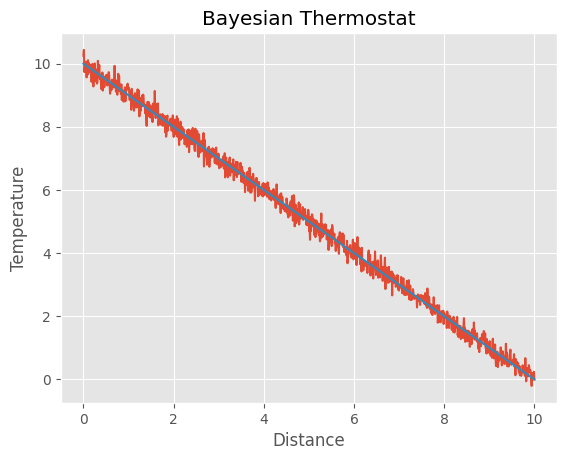
\includegraphics[scale=0.55]{images/bayesian_theromostat.png}
    \caption{Visualisation of the Bayesian Thermostat environment with the true line depicting the line $y = 10 - x$. While the red is a demonstration of the type of observations the agent would receive in the environment.}
    \label{fig:bayesian_thermostat}
\end{figure}

\subsubsection{Perception}

The problem of perception within the Bayesian Thermostat environment is inferring the distance the agent is from the heat source, given the noisy temperature readings generated by the environment. We need to define the generative model for the agent:

\begin{equation}\label{eq:bayesian_thermostat_generative_model}
	\begin{aligned}
		y | x &\sim N\left(f(x), \frac{1}{16}\right), \  x &\sim N\left(\bar{\mu}, \frac{1}{16}\right) ,\ f(x) &= 10 - x
	\end{aligned}
\end{equation}

Note the distinction in notation between $f$ which is a component of the generative model, and the underlying causal structure of the data generating process defined in \refp{eq:bayesian_thermostat}. That being said, for the purposes of perception, we have assumed the $f$ does indeed perfectly describe the underlying relation. Further, note that $f$ here is only a function of the neural activity and not the synaptic weight. This is because we are not considering learning yet, that will be treated in the next section. A final remark of $f$ - this is a function of the neural activity or hidden state $x$, but we will equally be considering it as a function of $\phi$. Since this is the posterior belief about this neural activity. So during inference $\phi$ will be the input to $f$. 

\

The final component of our generative model is the variational posterior distribution, we will be assuming this takes the form of a Dirac-delta distribution centred at $\phi$. Thus, can now derive the update equations for the hidden variable during inference in the Bayesian Thermostat environment from \refp{eq:pc_update_equations}: 

\begin{equation}\label{eq:pc_perception_phi}
	\begin{aligned}
		\frac{d \phi}{dt} = -\frac{\partial \mathcal{F}}{\partial \phi} &= \epsilon_y \frac{\partial f(\phi)}{\partial \phi} - \epsilon_x \\
		&= -\epsilon_y - \epsilon_x \\
    \end{aligned}
\end{equation}

During simulation we will update this hidden state using Euler's method, meaning we have some step size $\tau$ that is used to perform gradient on the VFE:

\begin{equation}
	\phi_{k + 1} = \phi_{k} + \tau \left( - \epsilon_y - \epsilon_x \right) 
\end{equation}

%NOTE: Need to work on this
A subtle point to note here is the different temporal scales we have introduced. $k$ denotes the time corresponding to the inference steps in the numerical implementation. Meaning that after convergence we update the hidden state for the environment time $t$. Precisely:

\begin{equation}
	x_{t + 1} = \phi_K
\end{equation}

Where $K$ denotes the inference steps that were needed for convergence. Which is a hyperparameter for the model, in this environment it was set at 10.

\

Suppose the agent's prior belief of its distance to the heat source, $\bar{\mu}$, is $4$. Meaning that the agent is expecting to observe a temperature reading of $f(9) = 6$. While further assume that the agent actually receives a temperature reading of $y = 2$. Meaning that it is likely that the agent is further from the heat source than its prior beliefs dictate. Indeed this is reflected in a plot of the inference steps \refp{fig:pc_example_perception}.

\begin{figure}[htbp]
    \centering
    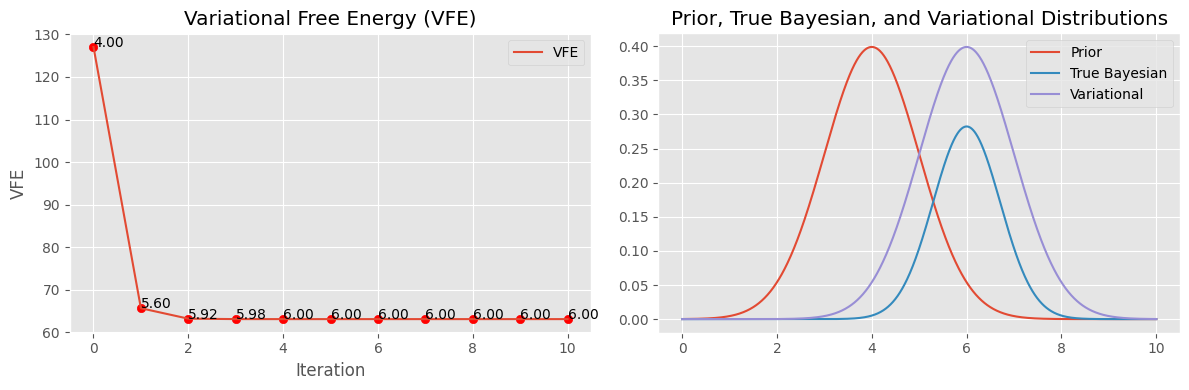
\includegraphics[scale=0.55]{images/pc_example_perception.png}
    \caption{Left: Plot of the the values of VFE during gradient descent. Each value plotted corresponds to the value of $\phi$ used in the calculation of the VFE. Right: After convergence of the $\phi$ we then use the parameter as the mean of our prior term in the generative model. This plot shows the difference between the prior distribution, the variational posterior and the true Bayesian posterior distribution. Important to note is that we are only performing gradient descent on the $\phi$ and simply keeping the variance of the prior distribution constant after convergence.}
    \label{fig:pc_example_perception}
\end{figure}

What we note about the inference plot in Figure \ref{fig:pc_example_perception} is that the variational posterior distribution does indeed correctly infer the true Bayesian posterior mean. The difference between these two distribution is due to the fact that we are not learning the variance of these distributions. You can refer to \citet{bogacz2017tutorial, friston2003learning} for demonstrations on this. It is also interesting to note for those not completely familiar with Bayesian inference, how the new mean of the distribution over hidden states is not the value that best describes the data, which in this case would be $x = 8$. But, the posterior beliefs represent a tradeoff between this optimal update and the priors beliefs about the hidden states.

\subsubsection{Learning}

We now aim to relax some of the assumptions that were made in the perception section. Namely, we will not assume that the agent has a perfect representation of the causal dynamics of the environment ie. we will assume that $f$ does not perfectly describe the relationship between the distance and the temperature. We will assume this function has the following form:

\begin{equation}
	f(x, \theta) = 10 - \theta x
\end{equation}

Practically, this means the model is required to not only infer where in the environment they are, but only learn the relation between where they are and the temperature. This is indeed somewhat circular, we require the dynamics to accurately infer where we are, but we need to know where we are to accurately infer the dynamics. This is the essential problem we are trying to solve. 

\

To learn and update the synaptic weights we will similarly use \refp{eq:pc_update_equations} to derive our update equations for $\theta$:

\begin{equation}\label{eq:theta_gradient_descent}
	\begin{aligned}
		\frac{d \theta}{dt} = - \frac{\partial \mathcal{F}}{\partial \theta}  &= \epsilon_y \frac{\partial f(\phi, \theta)}{\partial \theta} \\
		&= \eta \theta \epsilon_y
	\end{aligned}
\end{equation}

$\eta$ is the learning rate of the model. This is used to constrain the size of the update step in our weights. This is a common parameters used in machine learning neural networks and essentially boils down to the idea that the objective surface with respect to these synaptic weight is not well-behaved so we need to constrain the model to regulate its gradient descent. This parameters enters the model as a hyper-parameter that is set at $0.01$ in this example. We will similarly using Euler's method to update this parameters:


\begin{equation*}
	\theta_{t + 1} = \theta_{t} + \tau ( \eta \phi \epsilon_y )
\end{equation*}

Notice that this temporal scale is the environment's. Meaning that we will take a single gradient descent step with respect to the weight. We will also need to adjust the algorithm for hidden state inference given the generalisation of $f$:

\begin{equation}\label{eq:pc_learning_phi}
	\begin{aligned}
		\frac{d \phi}{dt} = -\frac{\partial \mathcal{F}}{\partial \phi} &= \epsilon_y \frac{\partial f(\phi, \theta)}{\partial \phi} - \epsilon_x \\
		&= \theta \epsilon_y - \epsilon_x \\
    \end{aligned}
\end{equation}

We assume the same prior and observation as the previous section. Only that we are now required to initialise the $\theta = -0.75$. We see the results from the inference scheme in \ref{fig:pc_example_learning}. 

\

\begin{figure}[htbp]
	\centering
	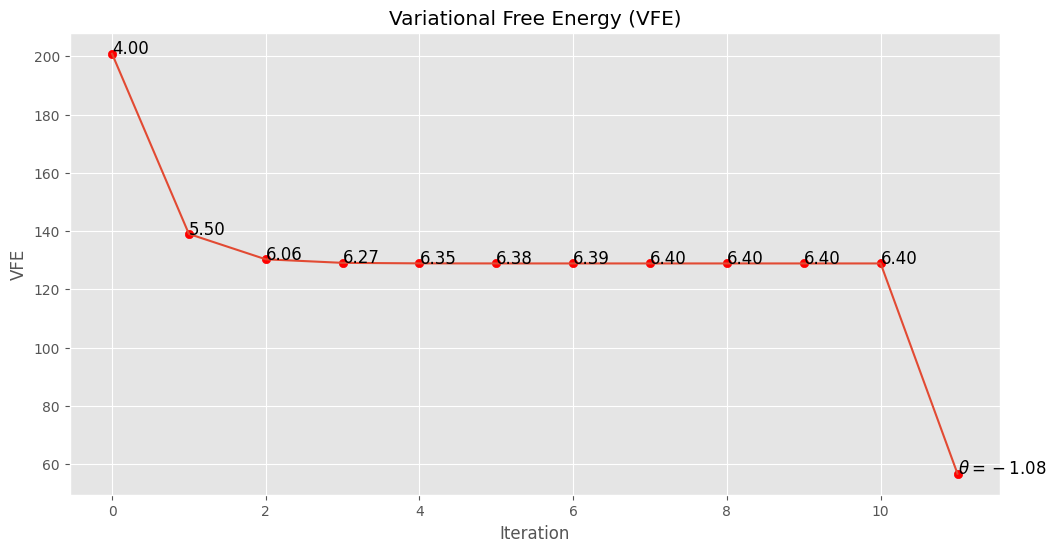
\includegraphics[scale=0.5]{images/pc_example_learning.png}
	\caption{The gradient descent on VFE that was described in the example of learning in predictive coding. The first 10 points demonstrate the descent with respect to $\phi$ and the final step is the step with respect to $\theta$ described in \refp{eq:theta_gradient_descent} With hyper-parameters of $\eta = 0.01$ and $\tau = 0.01$} 
	\label{fig:pc_example_learning}
\end{figure}

We observe that VFE converges to a value that is greater to the corresponding Figure \refp{fig:pc_example_perception} in the perception section. However, the (M) step in the (EM) scheme moves the VFE below what we see in perception. Moreover, we see that this step with respect $\theta$ actually overestimates the synaptic weight. (-1.08 compared to the true value -1) This is not a surprise since our converged hidden distance is 6.4. Which means that the temperature reading is actually better explained by a larger $\theta$ given our prior beliefs, therefore we overstep the true value. This is a good demonstration of how the inference is constraint by how well the model explains the environment. Since the agent is incorrect about both its distance and its belief of the relationship between the distance and the temperature we are naturally going to see instability in this inference.

\subsubsection{Planning}

The final component to our predictive coding model is planning. So far, what we have discussed has not referred to active inference, through as we saw in the previous section this notion of variational free energy minimisation is related to active inference. Predictive coding as we have described does not incorporate planning. For this, we will use active inference and specifically the EFE functional to define the distributions over policies. In this case, we will be considering a single time-step into the future which in the case of this simple environment is sufficient. 

\

The simplification that is made in this model of planning is the transitions. We will assume that the agent knows exactly how (its beliefs) of the distance to the heat source will change with each action. We define 3 actions that the agent can take: Left, right and stay. Further, we define the transition dynamics as Dirac-delta distributions:

\begin{equation}
\begin{aligned}
	P(x_{t+1} | x_t, u^S_{t+1}) &= \delta(x_{t+1} - x_t ) \\
	P(x_{t+1} | x_t, u^L_{t+1}) &= \delta(x_{t+1} - ( x_t - 0.01) ) \\
	P(x_{t+1} | x_t, u^R_{t+1}) &= \delta(x_{t+1} - ( x_t + 0.01) ) 
\end{aligned}
\end{equation}

Where $u^L$ is the move left action, $u^S$ is stay and $u^R$ is move right. These transitions mean that the agent will move 0.01 units right when the right action is taken. Similarly, for the left action. And will stay at the sample place with the stay action. 

\

As described in the previous section, the EFE is evaluated based on some preference distribution over actions. In this way we allow for the agent to be goal-directed. For this environment, we will again assume that the preference distribution is a Gaussian distribution over the observations:

\begin{equation}
	y | C \sim N(4, \frac{1}{16})
\end{equation}

This preference is completely arbitrary and is defined for demonstration. But we are now able to use these components to define the expected free energy for each action. Again, we will be choosing an alternative expression for the functional than what we saw in \ref{eq:efe}:

\begin{equation}\label{eq:efe_thermostat}
	\mathcal{G}(u_{t+1}) = \underbrace{\mathbb{E}_{Q(x_{t+1} | u_{t+1})} \left[ H[ P(y_{t+1} | x_{t+1}) ] \right]}_{\text{Ambiguity}} + \underbrace{D_{KL}\left[ Q(y_{t+1} | u_{t+1} \| P(y_{t+1} | C)) \right]}_{\text{Risk}}
\end{equation}

Let us now discuss each of these terms of how they are implemented in our scheme.

\

Ambiguity - This expression for EFE is particularly useful for Gaussian generative models since the entropy ($H(\cdot)$) of a normal distribution is only a function of the variance of the distribution not the mean. Since we are only considering learning of the mean this term becomes constant. Nevertheless, we have kept this term within the model since it will encourage exploration within the agent. This will become more clear when we demonstrate how exactly we create a distribution over the policies using EFE.

\

Risk - This is our expected divergence between the next observation and our preference distribution.

\

The EFE `values' each policy we are able to undertake, however, since we are assuming planning is as inference we will want to be able to sample from a distribution over the policy values to choose which action to take. To do this we will apply the softmax ($\sigma(\cdot)$) function to convert the EFE values for each policy into a distribution:

\begin{equation}
	P(\textbf{u}_{t+1}) = \sigma( - \mathcal{G}(\textbf{u}_{t+1}) )
\end{equation}

The softmax function will scale the vector input of actions into a distribution of actions proportional to the negative EFE. This makes sense since our aim is to minimise free energy. This is the why we have kept in the ambiguity constant, since this will increase the EFE of all actions equally it essentially saturates the proportional expected free energy of each action. Which in some instances may be detrimental to the performance of the model. However, we have found that this term allowed for more diverse actions selection initially which meant the agent learnt the dynamics of the environment in a more efficient way.

\

What we aim to demonstrate with planning is that the agent is able to consistently observe preferable temperature readings even in a noisy environment. What this means is that we need to dynamics of the agent to evolve over more than just a single time-step like we have so far. We have kept prior knowledge of distance consistent with prior sections, but we have set the true distance the agent is from the heat source as 8.\footnote{We have included a table of hyperparameters for this section and all previous section in Appendix \ref{appendix:hyperparameters}.} And allowed the agent to interact with the environment for 250 time-steps, with the results plotted in \ref{fig:pc_example_planning}. 

\begin{figure}[htbp]
	\centering
	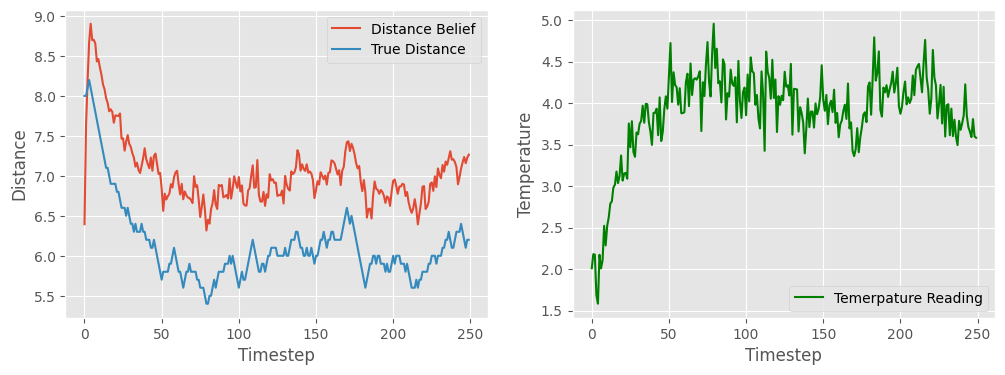
\includegraphics[scale=0.6]{images/pc_example_planning.png}
	\caption{Results of a predictive coding agent equipped with planning using EFE in the Bayesian Thermostat environment. Left: This depicts the difference between the agents belief of its distance to the heat source compared to the true distance it is from the heat source. We observe that the agent is consistently estimating its distance to be greater than the true distance. Right: This is a plot of the observations (temperature readings) observed by the agent over the episode. We notice that even though the agent did not have an accurate sense of where they were in the environment, they were able to consistently receive preferable observations. This is due to the fact that the dilution of the agent's own distance was offset by a weaker synaptic which in combination meant the agent converged to a reasonable niche within the environment.}
	\label{fig:pc_example_planning}
\end{figure}

\

We observe the agent consistently received preferable temperature readings from around 50 time-steps. The agent stays approximately in this niche until the end of the episode. In this sense, the agent has solved the environment. What is interesting however, is the distorted beliefs the agent has over its own distance. Throughout the episode there is a distinct difference between where the agent is compared to where it thinks it is. The reason the able to able to still `solve' the environment is that the range of synaptic weight offsets this distortion in some sense. The average weight over the last 200 time-steps is $-0.865$ and its average belief about its own distance over the same period is $6.9$. Meaning that based on the agent's beliefs of the dynamics of the environment it has solved the environment ($6.9 \times -0.865 + 10 = 4.03$). This could of course be avoided and there could be some additional component of the model at the other end - for example - that could force the agent to have a more accurate representation of the environment. But this result leads to two interesting points of conversation. 

\

The first we have touched on previously - it is difficult for this agent to both infer where it is and the dynamics of the environment where there is a degree of error in one. The circular nature of these components means that the agent can easily be placed in a situation where two wrongs make a right. Errors about the dynamics of the environment can cancel out with errors about its distance.

\

The second point I would like to note is that we have been referring to the $x$ variable as the agent's hidden belief about its own distance. But in reality, it is just a latent variable that needs to be inferred. We have placed it near enough and assumed other dynamics of the environment that push this variable to be `near' to the distance the agent is from the environment. But, if other components of the model were lifted and the relationship between the heat and the distance was more complicated. There would be more than one way to map a latent variable to the temperature reading. In such a situation the intuition of the latent variable as the distance would be lost. This leads to quite physiological conversation about how each of us represent our environment's internally. There is no guarantee that there is consistency between those latent representation and that is why communication about the environment itself is grounded in observations rather than internal states. But for the purposes of this report still, in reality this hidden state could represent anything in that way it could really represent nothing specifically, which will become more clear in the next section where the size of the hidden state is in fact a hyper-parameter. 


\subsection{Temporal Predictive Coding}

In our discussion thus far we have only considered a single hidden state and single observation dimension. This model was useful for demonstration about the internal dynamics of predictive coding as well as revealing some of the complexities that arise even in simple situations with the model we are considering. We aim now to extend our understanding of predictive coding models to incorporate a deeper hierarchical structure. \citep{friston2008hierarchical} We will then use the slightly more complicated formulation of the generative, and variational components of the model to define the core component for this implementation section - \textit{temporal predictive coding}. This model of predictive coding aims to incorporate the correlation of sensory data into the components of the model. Once again, predictive coding does not include the notion of planning so we will be extending with model using EFE in a very similar way to what we have done in the previous section.

\subsubsection{Hierarchical Predictive Coding}

The success of deep neural networks in machine learning have demonstrated that having hierarchical sets of latent variables is key to enabling methods to learn powerful abstractions and to handle intrinsically hierarchical dynamics of the sort humans intuitively perceive. The predictive coding schemes previously introduced can be straightforwardly extended to handle hierarchical dynamics of arbitrary depth, equivalently to deep neural networks in machine learning.

\

This is done by postulating multiple layers of latent variables, $x_1, \dots, x_L$ and defining the generative model as:

\begin{equation}
	p(x_0, \dots, x_L) = p(x_L) \prod_{l = 0}^{L - 1} p(x_l | x_{l-1})
\end{equation}

Where $x_l | x_{l - 1} \sim N(f_l(x_{l + 1}; \theta_{l + 1}) , \Sigma_l)$ and the final layer $x_L \sim N(\bar{x_L}, \Sigma_L)$ has some arbitrary prior $\bar{x_L}$ and the latent variable at the bottom of the hierarchy is set to what was actually observed $x_0 = y$. 

\

Similarly, we define a variational posterior for the generative model that can be decomposed for each layer:

\begin{equation}
	q(x_{1:L}) = \prod^L_{l = 1} \delta(x_l - \phi_l)
\end{equation}

The variational free energy can thus be written as the sum of prediction errors on each level:

\begin{equation}\label{eq:vfe_pc_hierarchical}
\mathcal{F} = \prod_{l = l}^{L} \Sigma_l^{-1} \epsilon_l^2 + \ln 2 \pi \Sigma_l
\end{equation}

Where $\epsilon_l = \phi_l - f_l(\theta_{l + 1}, \phi_{l + 1})$\footnote{Which is subtly different to the error in the previous section. This is simply notional, and is due to the difference between $\Sigma$ being the co-variance matrix while $\sigma$ is standard deviation.}

\

Since the free energy can be nicely divided into sum of layer-wise prediction errors, it is natural to express the dynamics of $\phi$ and $\theta$ in a similar way:

\begin{equation}
	\begin{aligned}
		\frac{d\phi_l}{dt} &= - \frac{\partial \mathcal{F}}{d\phi_l} = \Sigma_{l - 1}^{- 1} \epsilon_{l - 1} \frac{\partial f_{l - 1}}{\partial \phi_{l}} \theta_l^T - \Sigma_{l}^{-1} \epsilon_l \\
		\frac{d\theta_l}{dt} &= - \frac{\partial \mathcal{F}}{d\theta_l} = \Sigma_{l - 1}^{- 1} \epsilon_{l - 1} \frac{\partial f_{l - 1}}{\partial \theta_{l}} \phi_l
	\end{aligned}
\end{equation}

\subsubsection{Temporal Predictive Coding}

In our examples and models of predictive coding we have mostly been focussed on treated each sensory observation independently. The problem with this approach is that sensory observations are highly correlated through time. So an essential feature of any model of the brain is how the model is able to handle this dynamically changing and correlated data. We aim to demonstrate this through a predictive coding model called temporal predictive coding (tPC). 

\

The generative structure of the temporal predictive coding model is a hidden Markov model (HMM). This means that for every time-step $t$ there exists an observation $y_t$ that only depends on the underlying hidden state at that point in time, $x_t$. The hidden state only depends on the previous hidden state $x_{t-1}$. While this is the usually structure of a HMM, \citet{millidge2024temporal} compared the models performing to Kalman filter in a Bayesian filtering task, which required an additional control unit, $u_t$, which too effects the underlying state. See Figure \ref{fig:hmm} for the probabilistic graphical model of the described HMM. 

\

\begin{figure}[h]
    \centering
    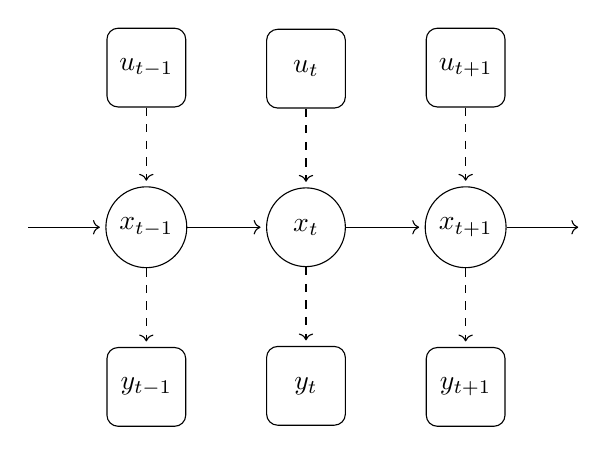
\begin{tikzpicture}[
        every node/.style={circle, draw, minimum size=1cm, node distance=1cm},
        state/.style={rectangle, rounded corners, draw, minimum size=1cm, node distance=1cm},
        ->, 
        shorten >=2pt, 
        auto
    ]

    % Hidden states
    \node (x1) at (0, 0) {$x_{t-1}$};
    \node (x2) [right=of x1] {$x_t$};
    \node (x3) [right=of x2] {$x_{t+1}$};

    % Controls
    \node[state] (u1) [above=of x1] {$u_{t-1}$};
    \node[state] (u2) [above=of x2] {$u_{t}$};
    \node[state] (u3) [above=of x3] {$u_{t+1}$};

    % Observations
    \node[state] (y1) [below=of x1] {$y_{t-1}$};
    \node[state] (y2) [below=of x2] {$y_{t}$};
    \node[state] (y3) [below=of x3] {$y_{t+1}$};

    % Transitions between hidden states
    \draw[->] (x1) to (x2);
    \draw[->] (x2) to (x3);
    
    % Actions
    \draw[->, dashed] (u1) -- (x1);
    \draw[->, dashed] (u2) -- (x2);
    \draw[->, dashed] (u3) -- (x3);
    
    % Emissions
    \draw[->, dashed] (x1) -- (y1);
    \draw[->, dashed] (x2) -- (y2);
    \draw[->, dashed] (x3) -- (y3);

    % Arrow from the left to x1
    \draw[->] ($(x1)+(-1.5, 0)$) -- (x1);

    % Arrow from x3 to the right
    \draw[->] (x3) -- ($(x3)+(1.5, 0)$);

    \end{tikzpicture}
    \caption{A Hidden Markov Model representation of the temporal predictive coding model (tPC). The model represents the recurrent connection between hidden states in the previous time step. The translations between hidden states are done by an activation on the previous level of activity, in this case this activation was a sigmoid function. The `transition' matrix A is then applied to these activated values, further the effect of a control input $u_t$ is applied to the value of each hidden state by a multiplication with the `control' matrix. The value of the hidden state is assumed to then generate the observations $y_t$. This emission is similarly done by passing hidden states through the activation function, with a weight matrix then applied to the output. Additionally, the emission component is equipped with a bias term in the model to scale the output to better represent the observations within the environment.}
    \label{fig:hmm}
\end{figure}

This model handles the correlation between sensory data by introducing the recurrent connection between hidden states. Machine learning and statistics have many established models with this recurrent connection established. Which include recurrent neural networks (RNN), and more advanced versions of RNN's like  Long Short-Term Memory (LSTM) models. However, for training these models use a method called backpropagation through time (BPTT). BPTT is considered to be biologically implausible because the brain processes inputs sequentially and in real time, and does not appear to have the ability to unfold sequences of computation through time. \citep{millidge2024temporal}

\

From the graphical model of the HMM we can write out specific equations for the dynamics of the states and observations in what is called the state-space representation:

\begin{equation}\label{eq:tpc}
	\begin{aligned}
		x_t &= A f(x_{t-1}) + B u_y + \omega_x \\
		y_t &= C f(x_t) + \omega_y
	\end{aligned}
\end{equation}

The $A$ matrix which we will call the `transition' matrix - encodes how the hidden states are expected to change from one time-step to the next. The $B$  encodes the effect of actions $u$ on the hidden states, which is called the `control' matrix. Finally the $C$ is the `emission' matrix translating the underlying state to observations. While $\omega_x, \omega_y$ are Gaussian noise. We can now translate this state-space representation into our tPC generative model:

\begin{equation}
\begin{aligned}
	x_t | x_{t-1}, u_{t} &\sim N( A f(x_{t-1} + B u_{t}), \Sigma_x) \\
	y_t | x_t &\sim N( C f(x_t) + c, \Sigma_y)
\end{aligned}
\end{equation}

The form of this generative model maps closely to the state-space representation. The only additional component that has been added is a bias term in the emission structure of the model, $c$. This term is not used in the original paper by \citet{millidge2024temporal}. Since this model was only used in filtering tasks scaling the output was not necessary. However, in our case, we will be using this model in a control task which does require the predicted output to be scaled to minimise the prediction error. Which from what we have seen in the previous section is very closely linked to the variational free energy which we are ultimately aiming to minimise in each observation. A bias term such as this is not needed in the temporal transition component of the model. This is due to the fact that the hidden states are not strictly trying to represent something physical. So the model will compute values that are valuable only within the context of the model, and therefore they do not need to be scaled to fit any data.

\

The other component of the model is the form of the activation function $f$. This function was chosen to be the sigmoid function, which is standard within the machine learning community. 

\

We will be assuming the Dirac-delta distribution as our variational posterior distribution, $q(x - \phi)$. We can then define the variational free energy objective:

\begin{equation}
    \begin{aligned}
        \mathcal{F} &= \frac{1}{2} \left(y_t - C f\left(x_t\right) - c\right)^T \Sigma_y^{-1} \left(y_t - C f\left(x_t\right) - c\right) \\
        &\quad + \frac{1}{2} \left(x_t - A f\left(\hat{x}_{t-1}\right) - B u_t\right)^T \Sigma_x^{-1} \left(x_t - A f\left(\hat{x}_{t-1}\right) - B u_t\right)
    \end{aligned}
\end{equation}

Still equipped with the assumption that the components of the model change over time to minimise the variational free energy. We are able to take the partial derivative of the free energy function to define our update equations:

\begin{equation}\label{eq:tpc_neural}
	-\frac{\partial \mathcal{F}}{\partial\phi_k}=-\epsilon_x+f^{\prime}\left(\phi_k\right) \odot C^T \epsilon_y
\end{equation}

We again note the temporal dynamics here. In the inference process we will be taking multiple gradient descent steps with respect to the posterior variational parameters. So, once $\phi$ has converged we will denote this as $\phi_K$. In which case the update is: $x_t = \phi_K$. We can take the partial derivative with respect to the other variables of interest:

\begin{equation}
    \begin{aligned}
        \Delta A &= -\eta \frac{\partial \mathcal{F}}{\partial A} = \eta \epsilon_x f\left(\hat{x}_{t-1}\right)^T \\
        \Delta B &= -\eta \frac{\partial \mathcal{F}}{\partial B} = \eta \epsilon_x u_t^T \\
        \Delta C &= -\eta \frac{\partial \mathcal{F}}{\partial C} = \eta \epsilon_y f\left(x_t\right)^T \\
        \Delta c &= -\eta \frac{\partial \mathcal{F}}{\partial c} = \eta \epsilon_y
    \end{aligned}
\end{equation}

Where $\epsilon_x := \Sigma_x^{-1}(x_t - A f(\hat{x}_{t-1}) - Bu_t)$ and $\epsilon_y := \Sigma_y^{-1}(y_t - C f(x_t) - c)$

\

These updates correspond to the (M) step in the EM scheme. We will again constrain the updates of our components by a learning rate, $\eta$, the dynamics of this hyper-parameters will be discussed later in this section. What is also to note is that $\hat{x_{t-1}}$ denotes the predicted hidden state in the previous time-step, while $x_t$ denotes the relaxed neural activity from the (E) step in \refp{eq:tpc_neural}. 

\subsubsection{Extending to Planning}

The extension to planning will happen in exactly the same fashion as the previous model. Meaning we will only be considering a policy of length one which means the model is only inferring what next action to perform. And similarly, we will be EFE with respect to each action and passing the negated value through the softmax function to create a distribution over actions that we then sample from to determine the next action. 

\

The departure from the previous model is that the agent is also tasked with learning the effects of its actions on the environment. This is represented in the model through the $B$ matix. The expected next state is then expressed as:

\begin{equation}
	x_{t+1} | u_t \sim N(A f(\hat{x}_{t}) + B u_{t}, \Sigma_x)
\end{equation}

We will then use the mean of this distribution, $\mu_{t+1} := A f(\hat{x}_{t}) + B u_{t}$ to create the distribution over observation in the next time-step:

\begin{equation}
	y_{t+1} | u_t \sim N( C f(\mu_{t+1}) + c, \Sigma_y)
\end{equation}

\subsubsection{Partially Observable Cart-Pole}

\begin{figure}[htbp]
    \centering
    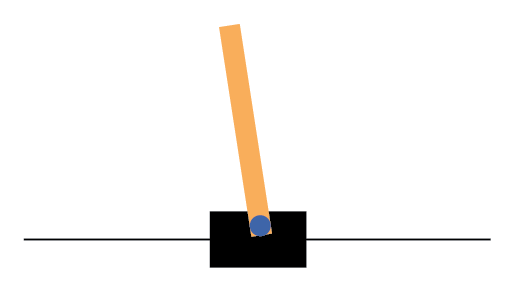
\includegraphics[scale=1.5]{images/cart_pole.png}
    \caption{A sample image from the OpenAI cart-pole environment}
    \label{fig:cart_pole}
\end{figure}

The cart-pole is a well-known environment used in reinforcement learning baselines. It requires controlling a cart with a pole attached, with the goal of balancing the pole upright. The environment typically provides observations such as the position and velocity of the cart, as well as the angle and angular velocity of the pole. However, since velocity naturally includes some temporal information, which our model is specifically designed to capture, we modified the OpenAI \citep{towers2024gymnasium} environment to reduce the observations to velocity only.

\

Furthermore, while the default environment assigns a reward at each time step, we redefined the objective to focus on maintaining the pole upright and the cart centred on the screen, similar to the approach taken by \citet{millidge2019combining}. This modification fundamentally changes the control problem, as the reward feedback is now much denser. Nonetheless, this variation presents a significantly greater challenge to the predictive coding model compared to previous environment.

\subsubsection{Results and Discussion}

\begin{figure}[htbp]
    \centering
    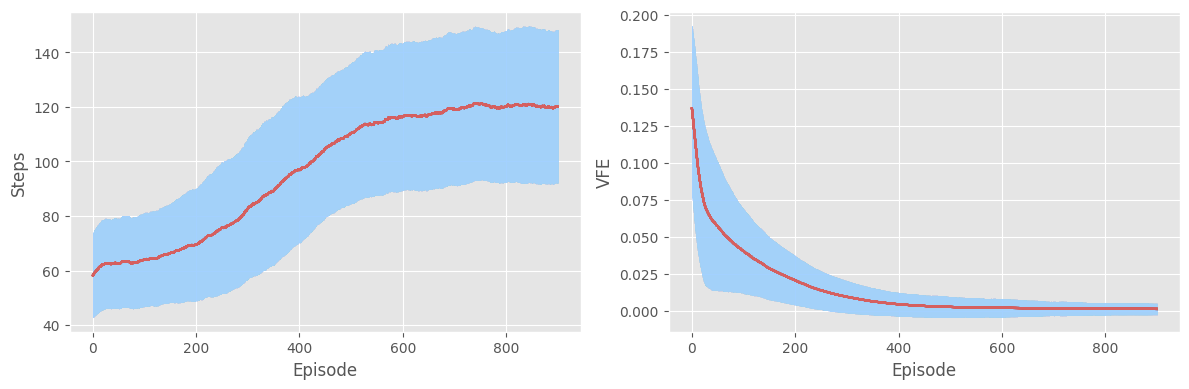
\includegraphics[scale=0.5]{images/tpc.png}
    \caption{Results of from the partially observable cart pole environment using temporal predictive coding with planning using expected free energy. \textbf{Left}: These are the averaged smoothed episodes steps across runs. The experiment used 25 runs with each one consisting of 1000 episodes, each of these runs were then smoothed using a 100 episode moving average, these moving averages themselves were then averaged together to give the red line. The blue area depicts a confidence interval for this average. This represents a single standard deviation from the average moving average. \textbf{Right}: This depicts the associated variational free energy to the left plot. Meaning that this depicts the red line depicts the average moving average of this variational free energy per episode. The VFE per episode consisted of averaging the free energy per observation. The blue area similarly depicts a single standard deviation from the mean.}
    \label{fig:tpc_results}
\end{figure}

The experiment involved 1000 episodes across 25 separate runs. The results are shown in Figure \refp{fig:tpc_results}. The plot on the left, which illustrates the number of steps the agent managed to balance the pole, shows a significant improvement after around 250 episodes, with the agent maintaining balance for over 120 time steps. This shows a non-trivial level of learning in this task. The baseline control rule, which is simply if the pole leans move left, is able to achieve an average of 50 time units \citep{millidge2019combining}. We can also notice a very clear correlation between the average variational free energy, depicted on the right, and the performance in the task. When the model is able to reduce the variational free energy of the observation, it is able to improve its performance. While, we notice that when the VFE converges to almost zero - the performance too plateaus. 

\

Further, the variance of the tPC model in its balance is very noisy. In particular runs the model was able to balance the pole for 500 time units (the maximum) while the next run it could drop back down to a balance of 50 units. In order to reduce the variance of this model we exponentially decayed the learning rate parameter $\eta$. While this did assist in the agent consistently achieving better results through the episode, it was unable to reduce the episode to episode variance. 

\

The natural question to ask is how well is the agent learning the dynamics of the environment. VFE is closely associated with this since as we have seen this is an upper bound on the surprise of the observation. But we are able to measure this more exactly using simply prediction error. If an agent is in a particular state and they choose to execute a certain action, part of that action selection process was to cast itself one step into the future. A process highlighted in the previous section. We can therefore compare how accurate this forecasting is. We did this by computing the norm of the predicted observation from the counterfactual process within the computation of the EFE, against the actual observation. These results are depicted in Figure \ref{fig:tpc_pred_error}. We observe that the prediction errors are clearly correlated with the variational free energy, which is of course expected, but what is interesting is that the model is unable to converge to zero prediction error. Meaning that it cannot fully model the dynamics of the environment. This is not unexpected since the dynamics of the cart-pole environment are fully modelled using a second-order dynamical system \citep{florian2005CorrectEF} which is difficult for a single layer network, even equipped with a with a non-linear activation function. 

\begin{figure}[htbp]
    \centering
        \begin{minipage}[c]{0.6\textwidth}
        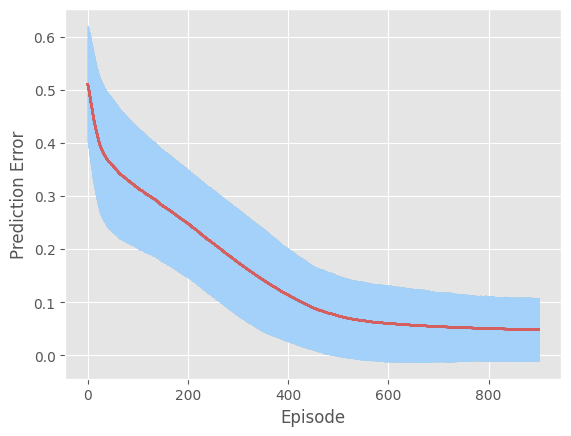
\includegraphics[width=\textwidth]{images/pred_error.png}
    \end{minipage}
    \hfill
    \begin{minipage}[c]{0.35\textwidth}
        \caption{The averaged moving average plot for the prediction errors in the experiment. The red line depicts the average moving average from the 25 runs across episodes, while the blue shaded region depicts a single standard deviation confidence interval.}
        \label{fig:tpc_pred_error}
    \end{minipage}
\end{figure}

\

As mentioned in the previous section, we cannot directly compare the results of this experiment with other cart-pole algorithms since the objective used in this model is a far more dense reward space. Nevertheless, \citet{millidge2024temporal} similarly used the observations from the environment to define the preference distribution for their active inference agent. Their model consisted of a hierarchical predictive coding model in the fully observable version of Cart-Pole. They were able to achieve an average of slightly less than 100 units across 50 trials.

%TODO: Compare these two models

\

An important point to note in this model is its sensitivity to initial conditions, particularly to the weight initialisation in the varies matrices. In some instances, a bad weight initialisation causes no learning across the 1000 episodes resulting in an average balancing steps of 9. Thus in our experiments we fixed the randomisation seed for weights across all runs. This problem is not indicative of a model that is unable to scale to more complex tasks, we note that deep neural networks suffer from a similar weight initialisation problem \citep{mishkin2016needgoodinit}. 


\subsection{Message Passing}

Predictive coding presents itself as a neural process theory. Meaning it is presenting a mechanistic explanation of cognitive functions and their neuronal underpinnings. However, for the processes of building active inference models\footnote{Active inference is also a process theory} predictive coding can be viewed as a variational inference algorithm for performing approximate Bayesian inference. Predictive coding is not unique in this respect, there are many such statistical inference algorithms that have been postulated to have a connection to neurobiology, one of them being \textit{message passing}.

\

In this report, we will be reviewing and implementing a message passing algorithm called \textit{belief propagation}. Belief propagation allows exact computation of marginal posteriors at the expense of the architectural simplicity of other message passing algorithms. (Eg. variational message passing) We will be focussing on message passing on Forney-style factor graphs (FFG), also called normal factor graphs. FFG present a graphical description of the relation between variables and factors within a joint probability distribution. Expressing a joint probability distribution as an FFG we will be able to derive message that are passed from nodes on the graph that allow us to perform efficient and exact Bayesian inference. (On graphs with no loops)

\subsubsection{Forney-style Factor Graphs and Belief Propagation}

A Forney-style factor graph (FFG) is a graphical representation of a factorised probabilistic model, where edges represent variables and nodes specify relations between them. The purpose of expressing a joint probability distribution as an FFG is to highlight dependencies between variables, facilitating more efficient inference. To illustrate this, consider a joint probability distribution of the form:

\begin{equation}\label{eq:ffg_inference_example}
	p(x_1, x_2, x_3) = \frac{1}{Z}f_a(x_1)f_b(x_1, x_2)f_c(x_2, x_3)
\end{equation}

\begin{figure}[h]
    \centering
	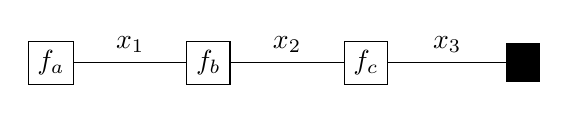
\begin{tikzpicture}[node distance=2cm, auto, ->, >=]

    	% Define nodes
	    \node (fa) [draw, rectangle] {$f_a$};
    	\node (fb) [draw, rectangle, right of=fa] {$f_b$};
	    \node (fc) [draw, rectangle, right of=fb] {$f_c$};
	    \node (d) [draw, rectangle, right of=fc, fill=black] {$d$};

	    % Draw arrows
    	\draw[->] (fa) -- node {$x_1$} (fb);
	    \draw[->] (fb) -- node {$x_2$} (fc);
    	\draw[->] (fc) -- node {$x_3$} (d);

	\end{tikzpicture}
	\caption{FFG for the joint probability distribution in \refp{eq:ffg_inference_example}. Each factor is displayed in block, with each variable represented as an edge in the graph. The observed variable is depicted as a black node, this represents the $\delta$ function to clamp the value of the variable $x_3$.}
	\label{fig:belief_propogation}
\end{figure}

Where $Z$ is a normalisation constant. Then let us consider the problem of inferring the marginal distribution of $x_2$ given some observation of $x_3$.

\begin{equation}
\begin{aligned}
	p(x_2 | x_3 = \widehat{x_3}) &\propto \int_{x_1, x_3} p(x_1, x_2, x_3) \delta(x_3 - \widehat{x_3}) \ dx_2 dx_3 \\
	&\propto \int_{x_1, x_3} f_a(x_1)f_b(x_1, x_2)f_c(x_2, x_3) \delta(x_3 - \widehat{x_3}) \ dx_2 dx_3
\end{aligned}
\end{equation}

We use the Dirac function, $\delta$, to clamp the variable to take the observed value. 

\

The key point is that not all factors (functions) depend on every variable, which enables us to 'push in' the integrals. This lets us express the posterior in terms of more easily computable components, or \textit{messages}.

\begin{equation}
\begin{aligned}
	p(x_2 | x_3 = \widehat{x_3}) &\propto \int_{x_1, x_3} f_a(x_1)f_b(x_1, x_2)f_c(x_2, x_3) \delta(x_3 - \widehat{x_3}) \ dx_1 dx_3 \\
	&\propto \overbrace{\int_{x_1}f_a(x_1)f_b(x_1, x_2)}^{\mu_{f_a \to x_2}} \ dx_1 \underbrace{\int_{x_3}f_c(x_2, x_3) \overbrace{\delta(x_3 - \widehat{x_3})}^{\mu_{x_3 \to f_c (x_3)}} \ dx_3}_{\mu_{f_c \to x_2}} \\
	&\propto \mu_{f_b \to x_2} \mu_{f_c \to x_2}
\end{aligned}
\end{equation}

%TODO: I think I can phrase this better
$\mu$ is what we call a message. In the FFG we will be exploring the factors, $f$, will also be probability distributions. This means that these messages can just be considered as unnormalised probability distributions - otherwise known as beliefs. Passing these messages around the factor graph is what gives rise to the notion of belief propagation.


\paragraph{Remark} The point that has not yet been address is the normalisation of these messages in order to form a valid probability distribution. This normalisation only requires the evaluation of low-dimensional integrals over local variables which makes it a more tractable computation. What is more, if all messages are Gaussian and any other node function is linear. The integrable has a closed form. \citep{bagaev2021reactive}

%TODO: I think I need to mention this - it might make more sense in the predictive coding section

\paragraph{Remark} This leads us to an important distinction between the falsifiable nature of the present argument. There appears to be done contradiction between the notion that we cannot perform Bayesian inference on large models because we cannot marginalise but we have just claimed that we can. This is because we are proposing a neural implementation that can be proved incorrect.

\paragraph{Equality Factor} Within a FFG we depict a variable as an edge connecting two factors. As opposed to a bipartite graph where they are depicted as nodes with edges corresponding to the relationship between variables and factors. This introduces a constraint that a variable can only be a function of two factors. We resolve this constraint by an equality factor. The equality factor resolves this situation by constraining the information about three variables to be equal. 	\citep{cox2019factor} More precisely:

\begin{equation}\label{eq:equality_factor}
	f_{=}(x, y, z) = \delta(x - z)\delta(x - y)
\end{equation}

Meaning that:

\begin{figure}[h]
    \centering
    \begin{minipage}{0.45\textwidth}
        \begin{equation*}
        \begin{aligned}
        	\mu_{\circled{3}}(z) &= \int \int \mu_{\circled{1}}(z) \mu_{\circled{2}}(z) \, dx_1 \, dx_2 \\
        	&= \mu_{\circled{1}}(z) \mu_{\circled{2}}(z)
        \end{aligned}
        \end{equation*}
    \end{minipage}
    \begin{minipage}{0.45\textwidth}
        \centering
        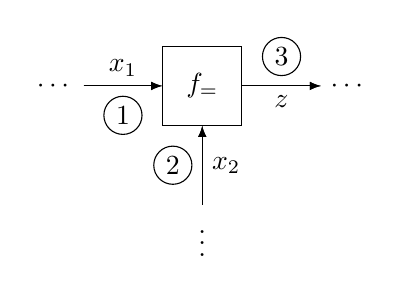
\begin{tikzpicture}[auto, node distance=1cm, >=latex]

            % Nodes
            \node (ldots) {$\cdots$};
            \node [right=of ldots] (equal) [draw, minimum size=1cm] {$f_=$};
            \node [right=of equal] (rdots) {$\cdots$}; % Three dots
            \node [below=of equal] (bdots) {$\vdots$};

            % Arrows and edge labels
            \draw[->] (ldots) -- node[above]{$x_1$}(equal);
            \draw[->] (ldots) -- node[below]{\circled{1}}(equal);

            \draw[->] (bdots) -- node[right]{$x_2$}(equal);
            \draw[->] (bdots) -- node[left]{\circled{2}}(equal);

            \draw[->] (equal) -- node[below]{$z$}(rdots);
            \draw[->] (equal) -- node[above]{\circled{3}}(rdots);

        \end{tikzpicture}
        \label{fig:equality_factor}
    \end{minipage}
    \caption{Example of the message passing behaviour over an equality factor}
\end{figure}

\subsubsection{Mountain Car}

%TODO: Mention more about this being an MDP, the observations modalities 

The mountain car environment describes an environment where a car is in a valley, and the car is not powerful enough to reach its target on the side of the mountain - higher up than it currently is. Thus the car is required to move backwards and generate enough force to then move to its target on the other side of the valley. 

\begin{figure}[htbp]
    \centering
    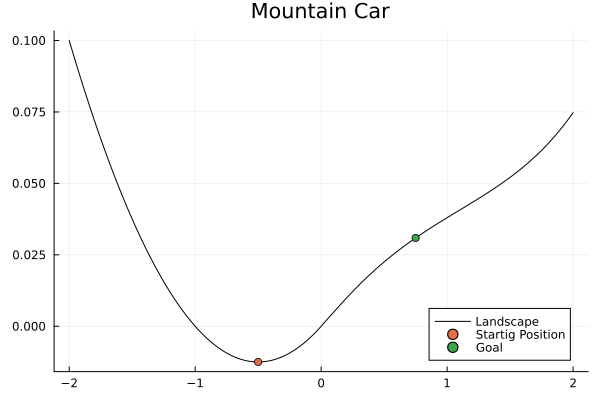
\includegraphics[scale=0.5]{images/mountain_car_plot.png}
    \caption{The landscape of the mountain car environment. Including the starting and target position for the model.}
    \label{fig:markov_blanket}
\end{figure}

\

This environment was originally proposed by \citet{moore90efficientmemory}, however the specific physics that are being used are based on the environment used in \citet{ueltzhoffer2018deep, van2019simulating}. Specifically, let us define the environmental states $z_t = (\phi_t, \dot{\phi}_t)$ depending on the position ($\phi_t$) and velocity of the car ($\dot{\phi}_t$). The environment is fully observable, meaning that the observations generated, $y_y$ , will be a reflection of these underlying states. The evolution of the state can then be described as:

\begin{equation}
	\begin{aligned}
		\dot{\phi}_t &= \dot{\phi}_{t-1} + F_g(\dot{\phi}_{t-1}) + F_f(\dot{\phi}_{t-1}) + F_a(a_t) \\
		\phi_t &= \phi_{t-1} + \dot{\phi}_t
	\end{aligned}
\end{equation}

Where $F_g$ is the gravitational force of the hill landscape that depends on the car's positions:

\begin{equation}
F_g(\phi) = \left\{
	\begin{aligned}
		&- 0.05 (2 \phi + 1), \ & \text{for } \phi < 0 \\
		&- 0.05 \left[ (1 + 5\phi^2 )^{-\frac{1}{2}} + \phi^2( 1 + 5\phi^2)^{-\frac{3}{2}} + \frac{1}{16} \phi^4\right] & \text{otherwise}
	\end{aligned}
	\right.
\end{equation}

$F_f$ is the friction of the car are is defined as $F_f(\dot{\phi}) = -0.1 \dot{\phi}$ and $F_a(a)$ is the engine force $F_a(a) = 0.04 \tanh(a)$ which restricts the force exerted by the car to be between -0.04 ad 0.04.

\subsubsection{Model}

Let us now define the form of the generative model. This model is derived from \citet{van2019simulating}, with some adjustment which will be highlighted. By using the Markov property of the environment we can define our generative model:

\begin{equation}\label{eq:mountain_car_generative_model}
	p_t(x, y, u) \propto p(x_{t-1}) \prod_{k=t}^{t + T} p(y_k | x_k) p(x_k | x_{k-1}, u_k)p(u_k)\tilde{p}(y_k)
\end{equation}

The Forney-factor graph for this generative model can be seen in Figure \ref{fig:online_ai_ffg}. The precise distributions defined for each component as:

\begin{equation}
\begin{aligned}
	p(y_k | x_k) &= N(x_k, \ \Sigma_y ) \\
	p(x_k | x_{k-1}, u_k) &= N(h(u_k) + g(x_{k-1}), \ \Sigma_x) \\
	p(u_k) &= N(0, \ \Sigma_u)
\end{aligned}	
\end{equation}

The component we have neglected to mention above is the preference distribution, within this model this component takes on a slightly different form. The model initialises the preference distribution as vague for the first $T$ time-steps. After which it is restricted to a concentrated distribution around the goal observation:

% TODO: Mention that there is not really any hidden states - MDP

\begin{equation}
	\tilde{p}(y_k) = \left\{
	\begin{aligned}
		& N((0, 0), \ 10^{4} \times \mathbb{I}_2) , \ & \text{for} \ k < T \\
		& N((0.75, 0), \ 10^{-4} \times \mathbb{I}_2) , \ & \text{otherwise}
	\end{aligned}
	\right.
\end{equation}

The algorithm for this model involves three steps each time-step:

\paragraph{1. Act-Execute-Observce} - We first select the \textbf{mean} of the marginal distribution over the controls, $u_k$. We then execute this actions on the environment and observe the new observations generated from the environment, $y_k$.

\paragraph{2. Infer} - Having executed a new action and generated a new observation at time $k$ we will then clamp these within the generative model and perform message passing to infer the posterior distribution of the generative model. This is the step where we require belief propagation.  

\paragraph{3. Slide} - In this step we instantiate the generative model by specifying the new prior to time $t+1$ as well sliding the inference horizon $T$. Specifically:

More specifically:


\begin{equation}
\begin{aligned}
    p_{t+1}(x, y, u) \propto 
    &\underbrace{\int \overbrace{p\left(x_{t-1}\right) p\left(x_t \mid x_{t-1}, u_t\right) p\left(y_t \mid x_t\right)}^{\text{first slice}} 
    \overbrace{\delta\left(u_t - \widehat{u_t}\right) \delta\left(y_t - \widehat{y_t}\right)}^{\text{action and observation}} dx_{t-1} du_t dy_t}_{\text{new prior - } p(x_t)} \\
    &\underbrace{\left(\prod_{k=t+1}^{t+T} p\left(x_k | x_k\right) p\left(x_k | x_{k-1}, u_k \right) p\left(u_k\right) \tilde{p}\left(y_k\right)\right)}_{\text{unaltered mid-section slices}} \\
    &\underbrace{p\left(y_{t+T+1} \mid x_{t+T+1}\right) p\left(x_{t+T+1} \mid x_{t+T}, u_{t+T+1}\right) p\left(u_{t+T+1}\right) \tilde{p}\left(y_{t+T+1}\right)}_{\text {add slice at horizon }}
\end{aligned}
\end{equation}

Upon inspection we can see that the new prior is nothing but the message coming from the equality node in Figure \ref{fig:online_ai_ffg}. 

\paragraph{Non-Linearity} The physical dynamics of the environment are not linear as described in the previous section. The issue with these non-linearities is that incoming messages from an exponential family of distributions is not guaranteed to be part of the exponential family when output. \citep{van2019simulating} Thus, we will perform a linear approximation of the change in hidden states over time as given by $F_g$ and $F_f$, this function is denoted as $g$. As well as a linear approximation of the control $F_a$ which is denoted $h$. The exact approximation technique was derived specifically for non-linearities in factor graphs \citep{petersen2018approximate}. 

\begin{figure}[h]
    \centering
\begin{tikzpicture}[auto, node distance=1cm, >=latex]

    % Nodes
    \node (dots) {$\cdots$}; % Three dots
    \node [right=of dots] (g) [draw, minimum size=1cm] {$g$};
    \node [right=of g] (plus) [draw, minimum size=1cm] {$+$};
    \node [right=of plus] (N) [draw, minimum size=1cm] {$p(x_k | x_{k-1}, u_k)s$};
    \node [right=of N] (equal) [draw, minimum size=1cm] {$=$};
    \node [right=of equal](dots1) {$\cdots$}; % Three dots

    \node [above=of plus] (h) [draw, minimum size=1cm] {$h$};
    \node [above=of h] (uk) [draw, minimum size=1cm] {$p(u_k)$};
    
    \node [below=of equal] (yk) [draw, minimum size=1cm] {$p(y_k | x_k)$};
    \node [below=of yk] (tilde_yk) [draw, minimum size=1cm] {$\tilde{p}(y_k)$};

    % Arrows and edge labels
    \draw[->] (dots) -- node[above] {$x_{k-1}$} (g);
    \draw[->] (g) -- (plus);
    \draw[->] (h) -- (plus);
    \draw[->] (uk) -- node[right]{$u_{k}$}(h);
    \draw[->] (plus) -- (N);
    \draw[->] (N) -- (equal);
    \draw[->] (equal) -- node[above]{$x_k$}(dots1);

    \draw[->] (equal) -- (yk);
    \draw[->] (yk) -- node[right]{$y_k$}(tilde_yk);

\end{tikzpicture}
\caption{A Forney-factor Graph for the generative model used in the mountain car environment. Each component will be repeated for each time along the time horizon $T$. The factors within the graph that denote the probability distributions have their arguments included in label. This is redundant since the edges dictate the arguments. This was done for clear reference to the generative model in \refp{eq:mountain_car_generative_model}.}
\label{fig:online_ai_ffg}
\end{figure}

\subsubsection{Results and Discussion}

All results in this environment were computed using the a package for Bayesian inference using message passing called RxInfer.jl \citep{bagaev2023rxinfer}. 

\begin{figure}[htbp]
    \centering
    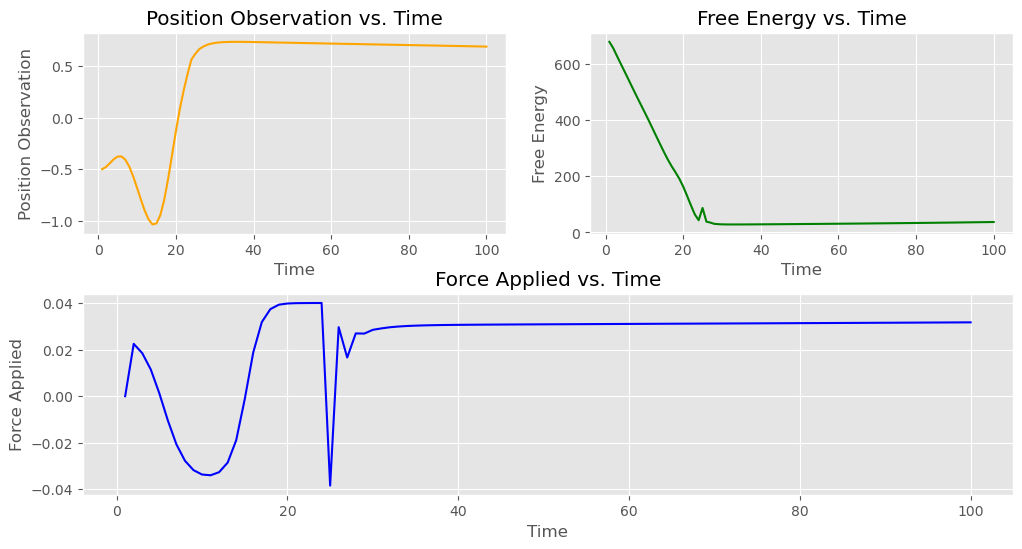
\includegraphics[scale=0.55]{images/mountain_car_results.png}
    \caption{Results from 100 time steps of the active inference agent experiment in the Mountain Car Environment. \textbf{Left}: This is a plot of the observations over the 100 time-steps. We see that the agent is able to reach the goal of a height of 0.75. \textbf{Right}: This is a plot of the force exerted by the agent over the course of the experiment. We observe that indeed the agent is able to move backwards to gain enough potential energy to reach its target height. }
    \label{fig:mountain_car_results}
\end{figure}

The results depicted in Figure \ref{fig:mountain_car_results} show that the active inference agent successfully reached its target height of 0.75 in the Mountain Car environment. To solve this challenge, the agent had to first move backward to gain enough potential energy, then use its forward momentum to climb high enough on the other side of the valley. This is evident in the force-over-time plot. Notably, the agent demonstrates awareness that gradually approaching the goal is not sufficient, and intelligently applies full forward force, followed by full backward force in a braking-like manoeuvre—a highly adaptive behaviour within this environment.

\

Some degree of exploration is clearly necessary within the environment. If the agent behaves greedily, applying full force directly towards the target, it fails to solve the problem. This is a limitation of the current model. By adjusting the variance of the preference distribution $\tilde{p}$ over time, we explicitly induce exploratory behaviour. In fact, if the agent is set with a strict preference distribution for the entire episode, it acts purely greedily and fails to solve the problem.

\

In theory, active inference provides an implicit solution to the exploration vs. exploitation dilemma. However, the current model does not compute actions based on the expected free energy (EFE) of each action; instead, actions are sampled from the mean of the marginal distribution. Modifying the model to incorporate this implicit exploration-exploitation tradeoff would be an intriguing direction for further research.


\subsubsection{Message passing and Neurobiology}

What is crucial to note is neural computations rely upon local connections across synapses. For a neuronal network to perform inference, it must integrate information from locally computed messages that are propagated among elements of that network \citep{parr2019neuronal}. 


\section{Conclusion}

\newpage

\bibliography{references}
\addcontentsline{toc}{section}{References}

\newpage

\appendix

\section{Hyperparameters}\label{appendix:hyperparameters}

\section{Gaussian Derivation}\label{appendix:laplace_approx}


\end{document}

